\documentclass[tikz,border=1pt]{standalone}
% Shared style of the Background schematics (bg_*.tex).  Colors follow figures/bar_patterns.py: each hue keeps one
% meaning across the paper (light blue with a blue outline = active / required position, green = WISEConv, red = the baseline
% frames, dotted gray = wasted computation, as in fig:gap).  Drawn at \columnwidth (241 pt), included unscaled.  Cell fills and
% the dark-navy rules come from the authors' original schematics (input C1E5F5, now a light lavender E2DCEE so that it stays apart from the blue active cells; weights a light yellow F6E2A6);
% the SM fill is a lighter step of their D9D9D9 so that it stays apart from the wasted gray.
\usepackage[T1]{fontenc}
\usepackage[tt=false,type1=true]{libertine}
\usepackage[libertine]{newtxmath}
\usepackage{tikz}
\usetikzlibrary{arrows.meta,calc,patterns.meta,positioning,fit,backgrounds,decorations.pathreplacing}

\definecolor{ink}{HTML}{222222}
\definecolor{muted}{HTML}{6B6B68}
\definecolor{rule}{HTML}{2A4552}
\definecolor{wiseconv}{HTML}{2A7F4A}
\definecolor{tileskip}{HTML}{5F7C97}
\definecolor{gather}{HTML}{7F98AF}
\definecolor{wasted}{HTML}{DDDDDD}
\definecolor{wastedink}{HTML}{9A9A9A}
\definecolor{baseline}{HTML}{C0392B}  % the baseline frames (red)
\definecolor{infill}{HTML}{E2DCEE}
\definecolor{wfill}{HTML}{F6E2A6}
\definecolor{smfill}{HTML}{EAEAEA}
\definecolor{actfill}{HTML}{D2E1F7}
\definecolor{actred}{HTML}{2A64C0}  % active positions: light blue fill, blue outline (2026-11-16 palette: green ours, red baselines, blue active)
\colorlet{gsfill}{gather!45!white}

\tikzset{
  every picture/.style={line join=round, line cap=round, font=\fontsize{8}{9.6}\selectfont, color=ink},
  cell/.style={draw=rule, line width=0.35pt, minimum size=#1, inner sep=0pt, outer sep=0pt, anchor=north west},
  cell/.default=3.6mm,
  idx/.style={font=\fontsize{6.8}{7}\selectfont, text=ink!85},
  act/.style={fill=actfill},
  inp/.style={fill=infill},
  wgt/.style={fill=wfill},
  waste/.style={fill=wasted, postaction={pattern={Dots[distance=1.2pt, radius=0.22pt]}, pattern color=wastedink}},
  gs/.style={fill=gsfill},
  sm/.style={fill=smfill, rounded corners=2pt, draw=none},
  mem/.style={fill=white, draw=rule, line width=0.4pt, rounded corners=1.2pt},
  smlabel/.style={font=\fontsize{6.8}{7}\selectfont\scshape, text=muted, anchor=north west, inner sep=1.4pt},
  flow/.style={-{Stealth[length=3.2pt, width=2.6pt]}, line width=0.55pt, draw=ink},
  title/.style={font=\fontsize{8}{9}\selectfont, anchor=north, inner sep=1pt},
  op/.style={font=\fontsize{9.5}{10}\selectfont, text=ink},
}

% \grid{x}{y}{cols}{rows}{size}{style of cell i (macro taking the index)}{first index label or empty}
% \actbox <path>; fills an active cell and outlines it in red on a layer above the grid lines
\pgfdeclarelayer{actlayer}
\pgfsetlayers{background,main,actlayer}
\def\actbox#1;{\fill[actfill] #1;\begin{pgfonlayer}{actlayer}\draw[actred, line width=0.6pt] #1;\end{pgfonlayer}}

\newcommand{\cellat}[4]{% x, y (top-left), size, style
  \node[cell=#3, #4] at (#1, #2) {};}

% \figframe{baseline|ours}{tag}: an outer frame around the whole schematic, placed last in the tikzpicture.  Baselines
% (fig:masked-conv, fig:tile-skip, fig:gather-scatter) get a dashed purple frame, WISEConv (fig:overview) a solid orange
% one, each with its tag on the top edge.  Colors and widths follow the frames of the intro figure (fig:teaser, purple
% Dense and orange WISEConv, 2026-11-15): both 0.9 pt, read off the figure at \columnwidth (about 5 px of 1280).
\tikzset{
  baselineframe/.style={draw=baseline, line width=0.9pt, dash pattern=on 2.4pt off 1.4pt, rounded corners=3pt},
  oursframe/.style={draw=wiseconv, line width=0.9pt, rounded corners=3pt},
  baselinetag/.style={fill=white, inner xsep=1.4pt, inner ysep=0.6pt, anchor=west, text=baseline!70!black,
                      font=\fontsize{7.4}{8}\selectfont\bfseries},
  ourstag/.style={baselinetag, text=wiseconv!80!black},
}
\newcommand{\figframe}[2]{%
  \coordinate (ff-sw) at ($(current bounding box.south west)+(-0.9,-0.9)$);
  \coordinate (ff-ne) at ($(current bounding box.north east)+(0.9,2.0)$);
  \draw[#1frame] (ff-sw) rectangle (ff-ne);
  \node[#1tag] at ($(ff-sw|-ff-ne)+(3.0,0)$) {#2};}

\usepackage[outline]{contour}\contourlength{0.9pt}
% fig:teaser.  Top: the (gray) driving frame x on the 12x5 grid of convolution positions, and the upstream mask M
% whose red cells are the active positions (grid and cells shared with teaser_assets.py).  Bottom: how each system
% executes the masked convolution.  Dense collects the 3x3 receptive field of every position into contiguous tiles
% (a 5x3 window shown, the rest elided); WISEConv collects only the active positions', laid out where they sit, from
% the same frame.  The width of each GPU box stands for its convolution time; the steering wheels on the timeline mark
% when planning finishes.
\definecolor{det}{HTML}{1F8A5B}
\definecolor{hood}{HTML}{E9EDF1}  % the ego vehicle's hood, as in figures/demo.png
\tikzset{
  detbox/.style={draw=det, line width=0.7pt},
  reused/.style={draw=det, line width=0.55pt, dash pattern=on 1.4pt off 0.9pt},
  small/.style={font=\fontsize{6.2}{7.0}\selectfont},
  stage/.style={draw=rule, line width=0.6pt, fill=white, rounded corners=1.5pt, align=center,
                font=\fontsize{6.4}{7.2}\selectfont, minimum width=8.8mm, minimum height=8.6mm, inner sep=0.9pt},
  wlabel/.style={font=\fontsize{7.4}{8}\selectfont\bfseries, fill=white, fill opacity=0.85, text opacity=1,
                 inner sep=0.8pt, rounded corners=1pt},
}
% detections in base-image pixels of the crop (x0, y0, x1, y1); \u is mm per pixel of the drawn copy
\def\detbus{(20*\u,-91*\u) rectangle (532*\u,-533*\u)}
\def\detman{(1300*\u,-241*\u) rectangle (1372*\u,-430*\u)}
\def\detped{(522*\u,-241*\u) rectangle (630*\u,-444*\u)}
\def\detcar{(718*\u,-276*\u) rectangle (818*\u,-356*\u)}
\newcommand{\wheel}[3]{% center, color, angle ranges of the steering arc's dashes (the last runs into the arrow) (as the trajectory in the scene:
  % outlined, dashed for Dense, one solid stroke for WISEConv); the arc turns clockwise, i.e. steering right
  \begin{scope}[shift={#1}]
    \draw[ink, line width=0.8pt] (0,0) circle (2); \fill[ink] (0,0) circle (0.5);
    \foreach \a in {90,210,330} \draw[ink, line width=0.7pt] (0,0) -- (\a:2);
    \fill[fill=#2] (45:2) circle (0.55);
    \foreach \a/\b/\e in {#3} {   % \e: angle by which the fill stops short of the dash's far end (0 where it meets the arrow)
      \draw[ink, line width=2.4pt, line cap=butt] (\a:3.1) arc[start angle=\a, end angle=\b, radius=3.1];
      \draw[draw=#2, line width=1.5pt, line cap=butt] ({\a-2.2}:3.1) arc[start angle={\a-2.2}, end angle={\b+\e}, radius=3.1];}
    \filldraw[fill=#2, draw=ink, line width=0.5pt, line join=round]
      ($(72:3.1)+(72:0.6)$) -- ($(72:3.1)+(-18:1.0)$) -- ($(72:3.1)+(252:0.6)$) -- cycle;
  \end{scope}}
\newcommand{\weights}[1]{% center of the 3x3 weights f, the size of one patch
  \begin{scope}[shift={#1}]
    \foreach \i in {0,1,2} \foreach \j in {0,1,2} \node[cell=0.6667mm, wgt, line width=0.25pt] at (-1+\i*0.6667, 1-\j*0.6667) {};
    \node[small, anchor=north] at (0,-1.2) {$\mathbf{f}$};
  \end{scope}}
\begin{document}
\begin{tikzpicture}[x=1mm, y=1mm]
  \def\W{85}\def\H{35.417}\def\s{7.0833}       % scene width, height, cell (1536x640 px, 128-px cells)
  \def\active{4/1,4/2,4/3,5/2,6/2}
  \def\p{2.2}\def\q{2.0}                          % patch pitch and size
  \def\ts{1.5833}\def\tw{19}\def\th{7.9167}\def\u{0.0123698}   % output thumbnail: cell, width, height, mm per pixel
  % ---------------- the frame x ----------------
  \node[anchor=north west, inner sep=0] at (0,0) {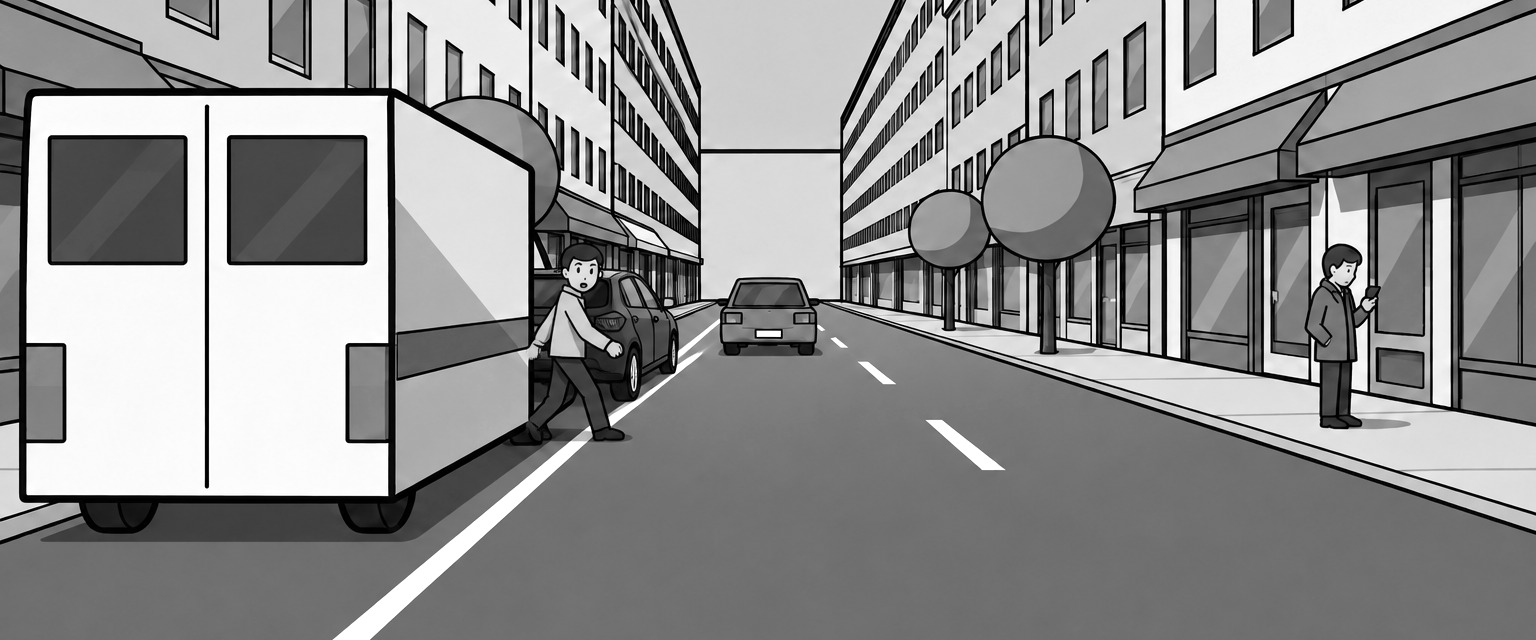
\includegraphics[width=\W mm]{teaser_assets/scene.jpg}};
  \foreach \c/\r in \active \fill[actfill, opacity=0.4] (\c*\s, -\r*\s) rectangle ++(\s, -\s);
  \foreach \k in {1,...,11} \draw[white, line width=0.5pt] (\k*\s, 0) -- ++(0, -\H);
  \foreach \k in {1,...,4} \draw[white, line width=0.5pt] (0, -\k*\s) -- ++(\W, 0);
  \foreach \c/\r in \active \draw[actred, line width=0.8pt] (\c*\s, -\r*\s) rectangle ++(\s, -\s);
  \draw[rule, line width=0.6pt] (0,0) rectangle (\W, -\H);
  % ego hood and trajectories, after the original teaser (figures/demo.png): Dense drives straight on until its
  % perception finishes (circle) and only then turns (dashed); WISEConv has already steered right
  \begin{scope}
    \clip (0,0) rectangle (\W,-\H);
    % generated by teaser_traj.py
\filldraw[fill=baseline, draw=ink, line width=0.55pt, line join=round] (41.311,-33.682) -- (41.315,-33.631) -- (41.319,-33.581) -- (41.323,-33.531) -- (41.326,-33.481) -- (41.330,-33.432) -- (41.334,-33.383) -- (41.337,-33.334) -- (41.341,-33.285) -- (41.345,-33.237) -- (41.348,-33.189) -- (41.352,-33.141) -- (41.355,-33.094) -- (41.359,-33.046) -- (41.363,-32.999) -- (41.366,-32.953) -- (41.370,-32.906) -- (41.373,-32.860) -- (41.376,-32.814) -- (41.380,-32.769) -- (41.383,-32.723) -- (41.387,-32.678) -- (41.390,-32.633) -- (41.393,-32.589) -- (41.397,-32.544) -- (41.400,-32.500) -- (41.403,-32.456) -- (41.407,-32.412) -- (41.410,-32.369) -- (41.413,-32.326) -- (41.416,-32.283) -- (41.419,-32.240) -- (41.423,-32.198) -- (41.426,-32.155) -- (41.429,-32.113) -- (41.432,-32.072) -- (41.435,-32.030) -- (41.438,-31.989) -- (41.441,-31.947) -- (41.445,-31.907) -- (41.448,-31.866) -- (41.451,-31.825) -- (41.454,-31.785) -- (41.457,-31.745) -- (41.460,-31.705) -- (41.463,-31.665) -- (41.466,-31.626) -- (41.468,-31.587) -- (41.471,-31.548) -- (41.474,-31.509) -- (41.477,-31.470) -- (41.480,-31.432) -- (41.483,-31.394) -- (41.486,-31.356) -- (41.489,-31.318) -- (41.491,-31.280) -- (41.494,-31.243) -- (41.497,-31.205) -- (41.500,-31.168) -- (41.503,-31.131) -- (41.505,-31.095) -- (41.508,-31.058) -- (41.511,-31.022) -- (41.514,-30.986) -- (41.516,-30.950) -- (41.519,-30.914) -- (41.522,-30.878) -- (41.524,-30.843) -- (41.527,-30.807) -- (41.530,-30.772) -- (41.532,-30.737) -- (41.535,-30.703) -- (41.537,-30.668) -- (41.540,-30.633) -- (41.543,-30.599) -- (41.545,-30.565) -- (41.548,-30.531) -- (41.550,-30.497) -- (41.553,-30.464) -- (41.555,-30.430) -- (41.558,-30.397) -- (43.642,-30.397) -- (43.645,-30.430) -- (43.647,-30.464) -- (43.650,-30.497) -- (43.652,-30.531) -- (43.655,-30.565) -- (43.657,-30.599) -- (43.660,-30.633) -- (43.663,-30.668) -- (43.665,-30.703) -- (43.668,-30.737) -- (43.670,-30.772) -- (43.673,-30.807) -- (43.676,-30.843) -- (43.678,-30.878) -- (43.681,-30.914) -- (43.684,-30.950) -- (43.686,-30.986) -- (43.689,-31.022) -- (43.692,-31.058) -- (43.695,-31.095) -- (43.697,-31.131) -- (43.700,-31.168) -- (43.703,-31.205) -- (43.706,-31.243) -- (43.709,-31.280) -- (43.711,-31.318) -- (43.714,-31.356) -- (43.717,-31.394) -- (43.720,-31.432) -- (43.723,-31.470) -- (43.726,-31.509) -- (43.729,-31.548) -- (43.732,-31.587) -- (43.734,-31.626) -- (43.737,-31.665) -- (43.740,-31.705) -- (43.743,-31.745) -- (43.746,-31.785) -- (43.749,-31.825) -- (43.752,-31.866) -- (43.755,-31.907) -- (43.759,-31.947) -- (43.762,-31.989) -- (43.765,-32.030) -- (43.768,-32.072) -- (43.771,-32.113) -- (43.774,-32.155) -- (43.777,-32.198) -- (43.781,-32.240) -- (43.784,-32.283) -- (43.787,-32.326) -- (43.790,-32.369) -- (43.793,-32.412) -- (43.797,-32.456) -- (43.800,-32.500) -- (43.803,-32.544) -- (43.807,-32.589) -- (43.810,-32.633) -- (43.813,-32.678) -- (43.817,-32.723) -- (43.820,-32.769) -- (43.824,-32.814) -- (43.827,-32.860) -- (43.830,-32.906) -- (43.834,-32.953) -- (43.837,-32.999) -- (43.841,-33.046) -- (43.845,-33.094) -- (43.848,-33.141) -- (43.852,-33.189) -- (43.855,-33.237) -- (43.859,-33.285) -- (43.863,-33.334) -- (43.866,-33.383) -- (43.870,-33.432) -- (43.874,-33.481) -- (43.877,-33.531) -- (43.881,-33.581) -- (43.885,-33.631) -- (43.889,-33.682) -- cycle;
\filldraw[fill=baseline, draw=ink, line width=0.55pt, line join=round] (41.644,-29.240) -- (41.647,-29.212) -- (41.649,-29.185) -- (41.651,-29.157) -- (41.653,-29.129) -- (41.655,-29.102) -- (41.657,-29.075) -- (41.659,-29.048) -- (41.661,-29.021) -- (41.663,-28.994) -- (41.665,-28.967) -- (41.667,-28.940) -- (41.669,-28.914) -- (41.671,-28.887) -- (41.673,-28.861) -- (41.675,-28.835) -- (41.677,-28.809) -- (41.679,-28.783) -- (41.681,-28.757) -- (41.683,-28.731) -- (41.685,-28.705) -- (41.687,-28.680) -- (41.688,-28.654) -- (41.690,-28.629) -- (41.692,-28.604) -- (41.694,-28.579) -- (41.696,-28.554) -- (41.698,-28.529) -- (41.700,-28.504) -- (41.702,-28.479) -- (41.703,-28.454) -- (41.705,-28.430) -- (41.707,-28.406) -- (41.709,-28.381) -- (41.711,-28.357) -- (41.713,-28.333) -- (41.714,-28.309) -- (41.716,-28.285) -- (41.718,-28.261) -- (41.720,-28.237) -- (41.721,-28.214) -- (41.723,-28.190) -- (41.725,-28.167) -- (41.727,-28.143) -- (41.728,-28.120) -- (41.730,-28.097) -- (41.732,-28.074) -- (41.734,-28.051) -- (41.735,-28.028) -- (41.737,-28.005) -- (41.739,-27.982) -- (41.741,-27.960) -- (41.742,-27.937) -- (41.744,-27.915) -- (41.746,-27.892) -- (41.747,-27.870) -- (41.749,-27.848) -- (41.751,-27.826) -- (41.752,-27.804) -- (41.754,-27.782) -- (41.755,-27.760) -- (41.757,-27.738) -- (41.759,-27.717) -- (41.760,-27.695) -- (41.762,-27.674) -- (41.764,-27.652) -- (41.765,-27.631) -- (41.767,-27.609) -- (41.768,-27.588) -- (41.770,-27.567) -- (41.772,-27.546) -- (41.773,-27.525) -- (41.775,-27.504) -- (41.776,-27.484) -- (41.778,-27.463) -- (41.779,-27.442) -- (41.781,-27.422) -- (41.782,-27.401) -- (41.784,-27.381) -- (41.785,-27.361) -- (43.415,-27.361) -- (43.416,-27.381) -- (43.418,-27.401) -- (43.419,-27.422) -- (43.421,-27.442) -- (43.422,-27.463) -- (43.424,-27.484) -- (43.425,-27.504) -- (43.427,-27.525) -- (43.428,-27.546) -- (43.430,-27.567) -- (43.432,-27.588) -- (43.433,-27.609) -- (43.435,-27.631) -- (43.436,-27.652) -- (43.438,-27.674) -- (43.440,-27.695) -- (43.441,-27.717) -- (43.443,-27.738) -- (43.445,-27.760) -- (43.446,-27.782) -- (43.448,-27.804) -- (43.449,-27.826) -- (43.451,-27.848) -- (43.453,-27.870) -- (43.454,-27.892) -- (43.456,-27.915) -- (43.458,-27.937) -- (43.459,-27.960) -- (43.461,-27.982) -- (43.463,-28.005) -- (43.465,-28.028) -- (43.466,-28.051) -- (43.468,-28.074) -- (43.470,-28.097) -- (43.472,-28.120) -- (43.473,-28.143) -- (43.475,-28.167) -- (43.477,-28.190) -- (43.479,-28.214) -- (43.480,-28.237) -- (43.482,-28.261) -- (43.484,-28.285) -- (43.486,-28.309) -- (43.487,-28.333) -- (43.489,-28.357) -- (43.491,-28.381) -- (43.493,-28.406) -- (43.495,-28.430) -- (43.497,-28.454) -- (43.498,-28.479) -- (43.500,-28.504) -- (43.502,-28.529) -- (43.504,-28.554) -- (43.506,-28.579) -- (43.508,-28.604) -- (43.510,-28.629) -- (43.512,-28.654) -- (43.513,-28.680) -- (43.515,-28.705) -- (43.517,-28.731) -- (43.519,-28.757) -- (43.521,-28.783) -- (43.523,-28.809) -- (43.525,-28.835) -- (43.527,-28.861) -- (43.529,-28.887) -- (43.531,-28.914) -- (43.533,-28.940) -- (43.535,-28.967) -- (43.537,-28.994) -- (43.539,-29.021) -- (43.541,-29.048) -- (43.543,-29.075) -- (43.545,-29.102) -- (43.547,-29.129) -- (43.549,-29.157) -- (43.551,-29.185) -- (43.553,-29.212) -- (43.556,-29.240) -- cycle;
\filldraw[fill=baseline, draw=ink, line width=0.55pt, line join=round] (41.839,-26.641) -- (41.841,-26.623) -- (41.842,-26.606) -- (41.843,-26.588) -- (41.845,-26.571) -- (41.846,-26.553) -- (41.847,-26.536) -- (41.849,-26.519) -- (41.850,-26.501) -- (41.851,-26.484) -- (41.852,-26.467) -- (41.854,-26.450) -- (41.855,-26.433) -- (41.856,-26.416) -- (41.858,-26.399) -- (41.859,-26.382) -- (41.860,-26.366) -- (41.861,-26.349) -- (41.863,-26.332) -- (41.864,-26.316) -- (41.865,-26.299) -- (41.866,-26.283) -- (41.868,-26.266) -- (41.869,-26.250) -- (41.870,-26.233) -- (41.871,-26.217) -- (41.872,-26.201) -- (41.874,-26.185) -- (41.875,-26.169) -- (41.876,-26.153) -- (41.877,-26.137) -- (41.878,-26.121) -- (41.880,-26.105) -- (41.881,-26.089) -- (41.882,-26.073) -- (41.883,-26.058) -- (41.884,-26.042) -- (41.886,-26.026) -- (41.887,-26.011) -- (41.888,-25.995) -- (41.889,-25.980) -- (41.890,-25.964) -- (41.891,-25.949) -- (41.892,-25.933) -- (41.894,-25.918) -- (41.895,-25.903) -- (41.896,-25.888) -- (41.897,-25.873) -- (41.898,-25.858) -- (41.899,-25.843) -- (41.900,-25.828) -- (41.902,-25.813) -- (41.903,-25.798) -- (41.904,-25.783) -- (41.905,-25.768) -- (41.906,-25.753) -- (41.907,-25.739) -- (41.908,-25.724) -- (41.909,-25.709) -- (41.910,-25.695) -- (41.911,-25.680) -- (41.913,-25.666) -- (41.914,-25.651) -- (41.915,-25.637) -- (41.916,-25.623) -- (41.917,-25.608) -- (41.918,-25.594) -- (41.919,-25.580) -- (41.920,-25.566) -- (41.921,-25.552) -- (41.922,-25.538) -- (41.923,-25.524) -- (41.924,-25.510) -- (41.925,-25.496) -- (41.926,-25.482) -- (41.927,-25.468) -- (41.928,-25.454) -- (41.929,-25.440) -- (41.930,-25.427) -- (41.932,-25.413) -- (43.268,-25.413) -- (43.270,-25.427) -- (43.271,-25.440) -- (43.272,-25.454) -- (43.273,-25.468) -- (43.274,-25.482) -- (43.275,-25.496) -- (43.276,-25.510) -- (43.277,-25.524) -- (43.278,-25.538) -- (43.279,-25.552) -- (43.280,-25.566) -- (43.281,-25.580) -- (43.282,-25.594) -- (43.283,-25.608) -- (43.284,-25.623) -- (43.285,-25.637) -- (43.286,-25.651) -- (43.287,-25.666) -- (43.289,-25.680) -- (43.290,-25.695) -- (43.291,-25.709) -- (43.292,-25.724) -- (43.293,-25.739) -- (43.294,-25.753) -- (43.295,-25.768) -- (43.296,-25.783) -- (43.297,-25.798) -- (43.298,-25.813) -- (43.300,-25.828) -- (43.301,-25.843) -- (43.302,-25.858) -- (43.303,-25.873) -- (43.304,-25.888) -- (43.305,-25.903) -- (43.306,-25.918) -- (43.308,-25.933) -- (43.309,-25.949) -- (43.310,-25.964) -- (43.311,-25.980) -- (43.312,-25.995) -- (43.313,-26.011) -- (43.314,-26.026) -- (43.316,-26.042) -- (43.317,-26.058) -- (43.318,-26.073) -- (43.319,-26.089) -- (43.320,-26.105) -- (43.322,-26.121) -- (43.323,-26.137) -- (43.324,-26.153) -- (43.325,-26.169) -- (43.326,-26.185) -- (43.328,-26.201) -- (43.329,-26.217) -- (43.330,-26.233) -- (43.331,-26.250) -- (43.332,-26.266) -- (43.334,-26.283) -- (43.335,-26.299) -- (43.336,-26.316) -- (43.337,-26.332) -- (43.339,-26.349) -- (43.340,-26.366) -- (43.341,-26.382) -- (43.342,-26.399) -- (43.344,-26.416) -- (43.345,-26.433) -- (43.346,-26.450) -- (43.348,-26.467) -- (43.349,-26.484) -- (43.350,-26.501) -- (43.351,-26.519) -- (43.353,-26.536) -- (43.354,-26.553) -- (43.355,-26.571) -- (43.357,-26.588) -- (43.358,-26.606) -- (43.359,-26.623) -- (43.361,-26.641) -- cycle;
\filldraw[fill=baseline, draw=ink, line width=0.55pt, line join=round] (41.968,-24.922) -- (41.969,-24.910) -- (41.970,-24.898) -- (41.971,-24.886) -- (41.972,-24.874) -- (41.973,-24.862) -- (41.974,-24.850) -- (41.975,-24.838) -- (41.976,-24.826) -- (41.976,-24.814) -- (41.977,-24.802) -- (41.978,-24.790) -- (41.979,-24.779) -- (41.980,-24.767) -- (41.981,-24.755) -- (41.982,-24.743) -- (41.983,-24.732) -- (41.983,-24.720) -- (41.984,-24.708) -- (41.985,-24.697) -- (41.986,-24.685) -- (41.987,-24.674) -- (41.988,-24.662) -- (41.989,-24.651) -- (41.990,-24.640) -- (41.990,-24.628) -- (41.991,-24.617) -- (41.992,-24.606) -- (41.993,-24.594) -- (41.994,-24.583) -- (41.995,-24.572) -- (41.995,-24.561) -- (41.996,-24.549) -- (41.997,-24.538) -- (41.998,-24.527) -- (41.999,-24.516) -- (42.000,-24.505) -- (42.000,-24.494) -- (42.001,-24.483) -- (42.002,-24.472) -- (42.003,-24.461) -- (42.004,-24.450) -- (42.005,-24.440) -- (42.005,-24.429) -- (42.006,-24.418) -- (42.007,-24.407) -- (42.008,-24.396) -- (42.009,-24.386) -- (42.009,-24.375) -- (42.010,-24.364) -- (42.011,-24.354) -- (42.012,-24.343) -- (42.013,-24.333) -- (42.013,-24.322) -- (42.014,-24.312) -- (42.015,-24.301) -- (42.016,-24.291) -- (42.016,-24.280) -- (42.017,-24.270) -- (42.018,-24.259) -- (42.019,-24.249) -- (42.020,-24.239) -- (42.020,-24.228) -- (42.021,-24.218) -- (42.022,-24.208) -- (42.023,-24.198) -- (42.023,-24.188) -- (42.024,-24.177) -- (42.025,-24.167) -- (42.026,-24.157) -- (42.026,-24.147) -- (42.027,-24.137) -- (42.028,-24.127) -- (42.029,-24.117) -- (42.029,-24.107) -- (42.030,-24.097) -- (42.031,-24.087) -- (42.032,-24.077) -- (42.032,-24.068) -- (42.033,-24.058) -- (43.167,-24.058) -- (43.168,-24.068) -- (43.168,-24.077) -- (43.169,-24.087) -- (43.170,-24.097) -- (43.171,-24.107) -- (43.171,-24.117) -- (43.172,-24.127) -- (43.173,-24.137) -- (43.174,-24.147) -- (43.174,-24.157) -- (43.175,-24.167) -- (43.176,-24.177) -- (43.177,-24.188) -- (43.177,-24.198) -- (43.178,-24.208) -- (43.179,-24.218) -- (43.180,-24.228) -- (43.180,-24.239) -- (43.181,-24.249) -- (43.182,-24.259) -- (43.183,-24.270) -- (43.184,-24.280) -- (43.184,-24.291) -- (43.185,-24.301) -- (43.186,-24.312) -- (43.187,-24.322) -- (43.187,-24.333) -- (43.188,-24.343) -- (43.189,-24.354) -- (43.190,-24.364) -- (43.191,-24.375) -- (43.191,-24.386) -- (43.192,-24.396) -- (43.193,-24.407) -- (43.194,-24.418) -- (43.195,-24.429) -- (43.195,-24.440) -- (43.196,-24.450) -- (43.197,-24.461) -- (43.198,-24.472) -- (43.199,-24.483) -- (43.200,-24.494) -- (43.200,-24.505) -- (43.201,-24.516) -- (43.202,-24.527) -- (43.203,-24.538) -- (43.204,-24.549) -- (43.205,-24.561) -- (43.205,-24.572) -- (43.206,-24.583) -- (43.207,-24.594) -- (43.208,-24.606) -- (43.209,-24.617) -- (43.210,-24.628) -- (43.210,-24.640) -- (43.211,-24.651) -- (43.212,-24.662) -- (43.213,-24.674) -- (43.214,-24.685) -- (43.215,-24.697) -- (43.216,-24.708) -- (43.217,-24.720) -- (43.217,-24.732) -- (43.218,-24.743) -- (43.219,-24.755) -- (43.220,-24.767) -- (43.221,-24.779) -- (43.222,-24.790) -- (43.223,-24.802) -- (43.224,-24.814) -- (43.224,-24.826) -- (43.225,-24.838) -- (43.226,-24.850) -- (43.227,-24.862) -- (43.228,-24.874) -- (43.229,-24.886) -- (43.230,-24.898) -- (43.231,-24.910) -- (43.232,-24.922) -- cycle;
\filldraw[fill=baseline, draw=ink, line width=0.55pt, line join=round] (42.100,-23.676) -- (42.104,-23.667) -- (42.108,-23.657) -- (42.112,-23.647) -- (42.117,-23.637) -- (42.121,-23.627) -- (42.126,-23.618) -- (42.131,-23.608) -- (42.135,-23.598) -- (42.140,-23.588) -- (42.146,-23.579) -- (42.151,-23.569) -- (42.156,-23.560) -- (42.162,-23.550) -- (42.167,-23.541) -- (42.173,-23.531) -- (42.179,-23.522) -- (42.185,-23.512) -- (42.191,-23.503) -- (42.197,-23.494) -- (42.203,-23.484) -- (42.210,-23.475) -- (42.216,-23.466) -- (42.223,-23.457) -- (42.229,-23.447) -- (42.236,-23.438) -- (42.243,-23.429) -- (42.250,-23.420) -- (42.257,-23.411) -- (42.264,-23.402) -- (42.272,-23.393) -- (42.279,-23.384) -- (42.287,-23.375) -- (42.294,-23.366) -- (42.302,-23.357) -- (42.310,-23.348) -- (42.318,-23.339) -- (42.326,-23.330) -- (42.334,-23.322) -- (42.342,-23.313) -- (42.350,-23.304) -- (42.359,-23.295) -- (42.367,-23.287) -- (42.376,-23.278) -- (42.384,-23.269) -- (42.393,-23.261) -- (42.402,-23.252) -- (42.411,-23.244) -- (42.420,-23.235) -- (42.429,-23.227) -- (42.438,-23.218) -- (42.447,-23.210) -- (42.456,-23.201) -- (42.466,-23.193) -- (42.475,-23.185) -- (42.485,-23.176) -- (42.495,-23.168) -- (42.504,-23.160) -- (42.514,-23.151) -- (42.524,-23.143) -- (42.534,-23.135) -- (42.544,-23.127) -- (42.554,-23.119) -- (42.564,-23.110) -- (42.575,-23.102) -- (42.585,-23.094) -- (42.595,-23.086) -- (42.606,-23.078) -- (42.616,-23.070) -- (42.627,-23.062) -- (42.638,-23.054) -- (42.649,-23.046) -- (42.659,-23.038) -- (42.670,-23.030) -- (42.681,-23.023) -- (42.692,-23.015) -- (43.592,-23.167) -- (43.583,-23.174) -- (43.574,-23.181) -- (43.565,-23.188) -- (43.557,-23.195) -- (43.548,-23.203) -- (43.540,-23.210) -- (43.532,-23.217) -- (43.523,-23.224) -- (43.515,-23.231) -- (43.507,-23.238) -- (43.499,-23.246) -- (43.491,-23.253) -- (43.483,-23.260) -- (43.475,-23.267) -- (43.468,-23.274) -- (43.460,-23.282) -- (43.453,-23.289) -- (43.445,-23.296) -- (43.438,-23.303) -- (43.431,-23.311) -- (43.423,-23.318) -- (43.416,-23.325) -- (43.409,-23.333) -- (43.402,-23.340) -- (43.395,-23.347) -- (43.389,-23.355) -- (43.382,-23.362) -- (43.375,-23.369) -- (43.369,-23.377) -- (43.363,-23.384) -- (43.356,-23.391) -- (43.350,-23.399) -- (43.344,-23.406) -- (43.338,-23.414) -- (43.332,-23.421) -- (43.326,-23.429) -- (43.320,-23.436) -- (43.314,-23.444) -- (43.309,-23.451) -- (43.303,-23.459) -- (43.298,-23.466) -- (43.293,-23.474) -- (43.287,-23.481) -- (43.282,-23.489) -- (43.277,-23.496) -- (43.272,-23.504) -- (43.267,-23.511) -- (43.263,-23.519) -- (43.258,-23.526) -- (43.253,-23.534) -- (43.249,-23.542) -- (43.245,-23.549) -- (43.240,-23.557) -- (43.236,-23.565) -- (43.232,-23.572) -- (43.228,-23.580) -- (43.224,-23.588) -- (43.220,-23.595) -- (43.217,-23.603) -- (43.213,-23.611) -- (43.210,-23.618) -- (43.206,-23.626) -- (43.203,-23.634) -- (43.200,-23.642) -- (43.197,-23.649) -- (43.194,-23.657) -- (43.191,-23.665) -- (43.188,-23.673) -- (43.186,-23.681) -- (43.183,-23.688) -- (43.181,-23.696) -- (43.178,-23.704) -- (43.176,-23.712) -- (43.174,-23.720) -- (43.172,-23.728) -- cycle;
\filldraw[fill=baseline, draw=ink, line width=0.55pt, line join=round] (43.093,-22.768) -- (43.105,-22.761) -- (43.118,-22.754) -- (43.132,-22.747) -- (43.145,-22.740) -- (43.158,-22.733) -- (43.171,-22.725) -- (43.185,-22.718) -- (43.198,-22.711) -- (43.212,-22.704) -- (43.225,-22.698) -- (43.239,-22.691) -- (43.252,-22.684) -- (43.266,-22.677) -- (43.280,-22.670) -- (43.294,-22.663) -- (43.307,-22.656) -- (43.321,-22.649) -- (43.335,-22.643) -- (43.349,-22.636) -- (43.363,-22.629) -- (43.377,-22.622) -- (43.391,-22.615) -- (43.405,-22.609) -- (43.419,-22.602) -- (43.433,-22.595) -- (43.448,-22.589) -- (43.462,-22.582) -- (43.476,-22.575) -- (43.491,-22.569) -- (43.505,-22.562) -- (43.519,-22.556) -- (43.534,-22.549) -- (43.548,-22.542) -- (43.563,-22.536) -- (43.577,-22.529) -- (43.592,-22.523) -- (43.607,-22.516) -- (43.621,-22.510) -- (43.636,-22.504) -- (43.651,-22.497) -- (43.666,-22.491) -- (43.680,-22.484) -- (43.695,-22.478) -- (43.710,-22.471) -- (43.725,-22.465) -- (43.740,-22.459) -- (43.755,-22.452) -- (43.770,-22.446) -- (43.785,-22.440) -- (43.800,-22.434) -- (43.815,-22.427) -- (43.830,-22.421) -- (43.846,-22.415) -- (43.861,-22.409) -- (43.876,-22.402) -- (43.891,-22.396) -- (43.907,-22.390) -- (43.922,-22.384) -- (43.937,-22.378) -- (43.953,-22.372) -- (43.968,-22.365) -- (43.984,-22.359) -- (43.999,-22.353) -- (44.729,-22.536) -- (44.714,-22.542) -- (44.700,-22.549) -- (44.686,-22.555) -- (44.672,-22.561) -- (44.658,-22.567) -- (44.644,-22.573) -- (44.630,-22.579) -- (44.616,-22.585) -- (44.602,-22.591) -- (44.588,-22.598) -- (44.574,-22.604) -- (44.561,-22.610) -- (44.547,-22.616) -- (44.533,-22.622) -- (44.519,-22.628) -- (44.506,-22.635) -- (44.492,-22.641) -- (44.479,-22.647) -- (44.465,-22.653) -- (44.452,-22.660) -- (44.438,-22.666) -- (44.425,-22.672) -- (44.412,-22.679) -- (44.399,-22.685) -- (44.385,-22.691) -- (44.372,-22.698) -- (44.359,-22.704) -- (44.346,-22.710) -- (44.333,-22.717) -- (44.320,-22.723) -- (44.307,-22.729) -- (44.294,-22.736) -- (44.281,-22.742) -- (44.269,-22.749) -- (44.256,-22.755) -- (44.243,-22.761) -- (44.231,-22.768) -- (44.218,-22.774) -- (44.206,-22.781) -- (44.193,-22.787) -- (44.181,-22.794) -- (44.168,-22.800) -- (44.156,-22.807) -- (44.144,-22.813) -- (44.132,-22.820) -- (44.120,-22.826) -- (44.107,-22.833) -- (44.095,-22.839) -- (44.083,-22.846) -- (44.072,-22.853) -- (44.060,-22.859) -- (44.048,-22.866) -- (44.036,-22.872) -- (44.024,-22.879) -- (44.013,-22.886) -- (44.001,-22.892) -- (43.990,-22.899) -- (43.978,-22.906) -- (43.967,-22.912) -- (43.956,-22.919) -- (43.944,-22.926) -- (43.933,-22.932) -- (43.922,-22.939) -- cycle;
\filldraw[fill=baseline, draw=ink, line width=0.55pt, line join=round] (44.443,-22.188) -- (44.459,-22.183) -- (44.475,-22.177) -- (44.491,-22.171) -- (44.507,-22.166) -- (44.524,-22.160) -- (44.540,-22.154) -- (44.556,-22.149) -- (44.573,-22.143) -- (44.589,-22.137) -- (44.605,-22.132) -- (44.622,-22.126) -- (44.638,-22.121) -- (44.654,-22.115) -- (44.671,-22.110) -- (44.687,-22.104) -- (44.704,-22.099) -- (44.720,-22.093) -- (44.736,-22.088) -- (44.753,-22.082) -- (44.769,-22.077) -- (44.786,-22.071) -- (44.802,-22.066) -- (44.819,-22.060) -- (44.835,-22.055) -- (44.852,-22.049) -- (44.869,-22.044) -- (44.885,-22.039) -- (44.902,-22.033) -- (44.918,-22.028) -- (44.935,-22.023) -- (44.952,-22.017) -- (44.968,-22.012) -- (44.985,-22.007) -- (45.002,-22.001) -- (45.018,-21.996) -- (45.035,-21.991) -- (45.052,-21.985) -- (45.068,-21.980) -- (45.085,-21.975) -- (45.102,-21.970) -- (45.118,-21.964) -- (45.135,-21.959) -- (45.152,-21.954) -- (45.169,-21.949) -- (45.186,-21.944) -- (45.202,-21.938) -- (45.219,-21.933) -- (45.236,-21.928) -- (45.253,-21.923) -- (45.269,-21.918) -- (45.286,-21.913) -- (45.303,-21.907) -- (45.320,-21.902) -- (45.337,-21.897) -- (45.354,-21.892) -- (46.008,-22.068) -- (45.991,-22.073) -- (45.975,-22.078) -- (45.959,-22.084) -- (45.943,-22.089) -- (45.926,-22.094) -- (45.910,-22.100) -- (45.894,-22.105) -- (45.878,-22.110) -- (45.862,-22.116) -- (45.846,-22.121) -- (45.830,-22.126) -- (45.814,-22.132) -- (45.798,-22.137) -- (45.782,-22.142) -- (45.766,-22.148) -- (45.749,-22.153) -- (45.733,-22.158) -- (45.718,-22.164) -- (45.702,-22.169) -- (45.686,-22.175) -- (45.670,-22.180) -- (45.654,-22.186) -- (45.638,-22.191) -- (45.622,-22.196) -- (45.606,-22.202) -- (45.590,-22.207) -- (45.574,-22.213) -- (45.559,-22.218) -- (45.543,-22.224) -- (45.527,-22.229) -- (45.511,-22.235) -- (45.496,-22.241) -- (45.480,-22.246) -- (45.464,-22.252) -- (45.449,-22.257) -- (45.433,-22.263) -- (45.417,-22.268) -- (45.402,-22.274) -- (45.386,-22.280) -- (45.371,-22.285) -- (45.355,-22.291) -- (45.340,-22.297) -- (45.324,-22.302) -- (45.309,-22.308) -- (45.293,-22.313) -- (45.278,-22.319) -- (45.263,-22.325) -- (45.247,-22.331) -- (45.232,-22.336) -- (45.217,-22.342) -- (45.201,-22.348) -- (45.186,-22.353) -- (45.171,-22.359) -- (45.156,-22.365) -- (45.140,-22.371) -- cycle;
\filldraw[fill=baseline, draw=ink, line width=0.55pt, line join=round] (45.793,-21.763) -- (45.810,-21.759) -- (45.827,-21.754) -- (45.844,-21.749) -- (45.861,-21.744) -- (45.878,-21.739) -- (45.895,-21.735) -- (45.912,-21.730) -- (45.929,-21.725) -- (45.945,-21.720) -- (45.962,-21.716) -- (45.979,-21.711) -- (45.996,-21.706) -- (46.013,-21.702) -- (46.030,-21.697) -- (46.047,-21.692) -- (46.064,-21.687) -- (46.081,-21.683) -- (46.098,-21.678) -- (46.115,-21.673) -- (46.132,-21.669) -- (46.148,-21.664) -- (46.165,-21.660) -- (46.182,-21.655) -- (46.199,-21.650) -- (46.216,-21.646) -- (46.233,-21.641) -- (46.250,-21.637) -- (46.267,-21.632) -- (46.284,-21.627) -- (46.300,-21.623) -- (46.317,-21.618) -- (46.334,-21.614) -- (46.351,-21.609) -- (46.368,-21.605) -- (46.385,-21.600) -- (46.401,-21.596) -- (46.418,-21.591) -- (46.435,-21.587) -- (46.452,-21.582) -- (46.469,-21.578) -- (46.485,-21.573) -- (46.502,-21.569) -- (46.519,-21.564) -- (46.536,-21.560) -- (46.553,-21.555) -- (46.569,-21.551) -- (46.586,-21.547) -- (46.603,-21.542) -- (46.620,-21.538) -- (46.636,-21.533) -- (46.653,-21.529) -- (47.274,-21.690) -- (47.257,-21.694) -- (47.241,-21.699) -- (47.224,-21.704) -- (47.208,-21.708) -- (47.192,-21.713) -- (47.175,-21.717) -- (47.159,-21.722) -- (47.142,-21.727) -- (47.126,-21.731) -- (47.109,-21.736) -- (47.093,-21.741) -- (47.076,-21.745) -- (47.060,-21.750) -- (47.043,-21.755) -- (47.027,-21.760) -- (47.010,-21.764) -- (46.994,-21.769) -- (46.977,-21.774) -- (46.961,-21.778) -- (46.944,-21.783) -- (46.928,-21.788) -- (46.911,-21.793) -- (46.895,-21.798) -- (46.878,-21.802) -- (46.862,-21.807) -- (46.845,-21.812) -- (46.829,-21.817) -- (46.812,-21.822) -- (46.796,-21.826) -- (46.779,-21.831) -- (46.763,-21.836) -- (46.746,-21.841) -- (46.730,-21.846) -- (46.713,-21.851) -- (46.697,-21.855) -- (46.680,-21.860) -- (46.663,-21.865) -- (46.647,-21.870) -- (46.630,-21.875) -- (46.614,-21.880) -- (46.597,-21.885) -- (46.581,-21.890) -- (46.565,-21.895) -- (46.548,-21.900) -- (46.532,-21.905) -- (46.515,-21.910) -- (46.499,-21.915) -- (46.482,-21.920) -- (46.466,-21.925) -- (46.449,-21.930) -- (46.433,-21.935) -- cycle;
\filldraw[fill=baseline, draw=ink, line width=0.55pt, line join=round] (46.162,-21.403) -- (48.046,-21.312) -- (47.824,-21.831) -- cycle;
\filldraw[fill=baseline, draw=ink, line width=0.55pt, line join=round] (43.615,-24.310) -- (43.600,-24.256) -- (43.567,-24.203) -- (43.519,-24.153) -- (43.456,-24.106) -- (43.380,-24.063) -- (43.292,-24.024) -- (43.193,-23.991) -- (43.085,-23.963) -- (42.970,-23.941) -- (42.850,-23.925) -- (42.726,-23.915) -- (42.600,-23.912) -- (42.474,-23.915) -- (42.350,-23.925) -- (42.230,-23.941) -- (42.115,-23.963) -- (42.007,-23.991) -- (41.908,-24.024) -- (41.820,-24.063) -- (41.744,-24.106) -- (41.681,-24.153) -- (41.633,-24.203) -- (41.600,-24.256) -- (41.585,-24.310) -- (41.586,-24.365) -- (41.605,-24.420) -- (41.642,-24.474) -- (41.696,-24.525) -- (41.767,-24.574) -- (41.854,-24.618) -- (41.954,-24.658) -- (42.068,-24.691) -- (42.191,-24.718) -- (42.323,-24.737) -- (42.460,-24.749) -- (42.600,-24.753) -- (42.740,-24.749) -- (42.877,-24.737) -- (43.009,-24.718) -- (43.132,-24.691) -- (43.246,-24.658) -- (43.346,-24.618) -- (43.433,-24.574) -- (43.504,-24.525) -- (43.558,-24.474) -- (43.595,-24.420) -- (43.614,-24.365) -- cycle;
\filldraw[fill=wiseconv, draw=ink, line width=0.55pt, line join=round] (41.483,-33.682) -- (41.489,-33.591) -- (41.495,-33.501) -- (41.501,-33.413) -- (41.506,-33.325) -- (41.512,-33.238) -- (41.518,-33.152) -- (41.523,-33.067) -- (41.529,-32.983) -- (41.534,-32.899) -- (41.539,-32.817) -- (41.545,-32.735) -- (41.550,-32.654) -- (41.555,-32.574) -- (41.560,-32.494) -- (41.565,-32.416) -- (41.571,-32.338) -- (41.576,-32.261) -- (41.580,-32.185) -- (41.585,-32.109) -- (41.590,-32.034) -- (41.595,-31.960) -- (41.600,-31.887) -- (41.605,-31.814) -- (41.609,-31.742) -- (41.614,-31.671) -- (41.619,-31.600) -- (41.623,-31.530) -- (41.628,-31.460) -- (41.632,-31.392) -- (41.636,-31.324) -- (41.641,-31.256) -- (41.645,-31.189) -- (41.650,-31.123) -- (41.654,-31.057) -- (41.658,-30.992) -- (41.662,-30.927) -- (41.666,-30.864) -- (41.670,-30.800) -- (41.675,-30.737) -- (41.679,-30.675) -- (41.683,-30.613) -- (41.687,-30.552) -- (41.691,-30.491) -- (41.694,-30.431) -- (41.698,-30.372) -- (41.702,-30.312) -- (41.706,-30.254) -- (41.710,-30.196) -- (41.714,-30.138) -- (41.717,-30.081) -- (41.721,-30.024) -- (41.725,-29.968) -- (41.728,-29.912) -- (41.732,-29.857) -- (41.735,-29.802) -- (41.739,-29.748) -- (41.742,-29.694) -- (41.746,-29.640) -- (41.749,-29.587) -- (41.753,-29.534) -- (41.756,-29.482) -- (41.760,-29.430) -- (41.763,-29.379) -- (41.766,-29.328) -- (41.769,-29.277) -- (41.773,-29.227) -- (41.776,-29.177) -- (41.779,-29.128) -- (41.783,-29.076) -- (41.787,-29.023) -- (41.792,-28.969) -- (41.798,-28.916) -- (41.804,-28.863) -- (41.812,-28.811) -- (41.820,-28.759) -- (41.828,-28.708) -- (41.838,-28.658) -- (41.848,-28.607) -- (41.859,-28.557) -- (41.870,-28.508) -- (41.882,-28.459) -- (41.895,-28.410) -- (41.908,-28.362) -- (41.922,-28.315) -- (41.936,-28.267) -- (41.952,-28.220) -- (41.967,-28.174) -- (41.984,-28.128) -- (42.000,-28.082) -- (42.018,-28.037) -- (42.036,-27.992) -- (42.054,-27.948) -- (42.073,-27.904) -- (42.092,-27.860) -- (42.112,-27.816) -- (42.132,-27.773) -- (42.153,-27.731) -- (42.175,-27.689) -- (42.196,-27.647) -- (42.219,-27.605) -- (42.241,-27.564) -- (42.264,-27.523) -- (42.288,-27.483) -- (42.312,-27.442) -- (42.336,-27.403) -- (42.361,-27.363) -- (42.386,-27.324) -- (42.411,-27.285) -- (42.437,-27.246) -- (42.463,-27.208) -- (42.490,-27.170) -- (42.517,-27.132) -- (42.544,-27.095) -- (42.572,-27.058) -- (42.600,-27.021) -- (42.628,-26.985) -- (42.656,-26.949) -- (42.685,-26.913) -- (42.715,-26.877) -- (42.744,-26.842) -- (42.774,-26.807) -- (42.804,-26.772) -- (42.834,-26.737) -- (42.865,-26.703) -- (42.896,-26.669) -- (42.927,-26.635) -- (42.958,-26.602) -- (42.990,-26.568) -- (43.022,-26.535) -- (43.054,-26.503) -- (43.086,-26.470) -- (43.119,-26.438) -- (43.152,-26.406) -- (43.185,-26.374) -- (43.218,-26.342) -- (43.252,-26.311) -- (43.286,-26.280) -- (43.319,-26.249) -- (43.354,-26.218) -- (43.388,-26.187) -- (43.422,-26.157) -- (43.457,-26.127) -- (43.492,-26.097) -- (43.527,-26.067) -- (43.562,-26.038) -- (43.598,-26.009) -- (43.633,-25.980) -- (43.669,-25.951) -- (43.705,-25.922) -- (43.741,-25.894) -- (43.777,-25.865) -- (43.814,-25.837) -- (43.850,-25.809) -- (43.887,-25.781) -- (43.924,-25.754) -- (43.961,-25.726) -- (43.998,-25.699) -- (44.035,-25.672) -- (44.072,-25.645) -- (44.110,-25.619) -- (44.147,-25.592) -- (44.185,-25.566) -- (44.223,-25.540) -- (44.261,-25.514) -- (44.299,-25.488) -- (44.337,-25.462) -- (44.375,-25.437) -- (44.413,-25.411) -- (44.452,-25.386) -- (44.490,-25.361) -- (44.529,-25.336) -- (44.568,-25.311) -- (44.606,-25.287) -- (44.645,-25.262) -- (44.684,-25.238) -- (44.723,-25.214) -- (44.762,-25.190) -- (44.801,-25.166) -- (44.841,-25.142) -- (44.880,-25.118) -- (44.919,-25.095) -- (44.959,-25.071) -- (44.998,-25.048) -- (45.038,-25.025) -- (45.077,-25.002) -- (45.117,-24.979) -- (45.157,-24.957) -- (45.196,-24.934) -- (45.236,-24.912) -- (45.276,-24.890) -- (45.316,-24.867) -- (45.356,-24.845) -- (45.396,-24.823) -- (45.436,-24.802) -- (45.476,-24.780) -- (45.516,-24.758) -- (45.556,-24.737) -- (45.596,-24.716) -- (45.636,-24.694) -- (45.677,-24.673) -- (45.717,-24.652) -- (45.757,-24.632) -- (45.797,-24.611) -- (45.837,-24.590) -- (45.878,-24.570) -- (45.918,-24.549) -- (45.958,-24.529) -- (45.999,-24.509) -- (46.039,-24.489) -- (46.079,-24.469) -- (46.119,-24.449) -- (46.160,-24.429) -- (46.200,-24.409) -- (46.240,-24.390) -- (46.281,-24.370) -- (46.321,-24.351) -- (46.361,-24.332) -- (46.402,-24.313) -- (46.442,-24.293) -- (46.482,-24.274) -- (46.522,-24.256) -- (46.563,-24.237) -- (46.603,-24.218) -- (46.643,-24.200) -- (46.683,-24.181) -- (46.723,-24.163) -- (46.763,-24.144) -- (46.804,-24.126) -- (46.844,-24.108) -- (46.884,-24.090) -- (46.924,-24.072) -- (46.964,-24.054) -- (47.004,-24.036) -- (47.044,-24.019) -- (47.083,-24.001) -- (47.123,-23.983) -- (47.163,-23.966) -- (47.203,-23.949) -- (47.243,-23.931) -- (47.282,-23.914) -- (47.322,-23.897) -- (47.362,-23.880) -- (47.401,-23.863) -- (47.441,-23.846) -- (47.480,-23.830) -- (47.520,-23.813) -- (47.559,-23.796) -- (47.598,-23.780) -- (47.638,-23.763) -- (47.677,-23.747) -- (47.716,-23.730) -- (47.755,-23.714) -- (47.794,-23.698) -- (47.833,-23.682) -- (47.872,-23.666) -- (47.911,-23.650) -- (47.950,-23.634) -- (47.988,-23.618) -- (48.027,-23.603) -- (48.066,-23.587) -- (48.104,-23.571) -- (48.143,-23.556) -- (48.181,-23.540) -- (48.219,-23.525) -- (48.258,-23.510) -- (48.296,-23.495) -- (48.334,-23.479) -- (48.372,-23.464) -- (48.410,-23.449) -- (48.448,-23.434) -- (48.485,-23.419) -- (48.523,-23.405) -- (48.561,-23.390) -- (48.598,-23.375) -- (48.636,-23.360) -- (48.673,-23.346) -- (48.710,-23.331) -- (48.748,-23.317) -- (48.785,-23.303) -- (48.822,-23.288) -- (48.859,-23.274) -- (48.896,-23.260) -- (48.932,-23.246) -- (48.969,-23.232) -- (49.006,-23.218) -- (49.042,-23.204) -- (49.079,-23.190) -- (49.115,-23.176) -- (49.151,-23.162) -- (49.187,-23.148) -- (49.223,-23.135) -- (49.259,-23.121) -- (49.295,-23.108) -- (49.331,-23.094) -- (49.366,-23.081) -- (49.402,-23.067) -- (49.437,-23.054) -- (49.472,-23.041) -- (49.508,-23.027) -- (49.543,-23.014) -- (49.578,-23.001) -- (49.613,-22.988) -- (49.647,-22.975) -- (49.682,-22.962) -- (49.717,-22.949) -- (49.751,-22.936) -- (49.785,-22.924) -- (49.820,-22.911) -- (49.854,-22.898) -- (49.888,-22.886) -- (49.921,-22.873) -- (49.955,-22.860) -- (49.989,-22.848) -- (50.022,-22.836) -- (50.056,-22.823) -- (50.089,-22.811) -- (50.122,-22.799) -- (50.155,-22.786) -- (50.188,-22.774) -- (50.221,-22.762) -- (50.254,-22.750) -- (50.286,-22.738) -- (50.319,-22.726) -- (50.351,-22.714) -- (50.383,-22.702) -- (50.415,-22.690) -- (50.447,-22.678) -- (50.479,-22.667) -- (50.511,-22.655) -- (50.542,-22.643) -- (50.574,-22.632) -- (50.605,-22.620) -- (50.636,-22.609) -- (50.667,-22.597) -- (50.698,-22.586) -- (50.729,-22.574) -- (50.760,-22.563) -- (50.790,-22.552) -- (50.821,-22.540) -- (50.851,-22.529) -- (50.881,-22.518) -- (50.911,-22.507) -- (50.941,-22.496) -- (50.971,-22.485) -- (51.000,-22.474) -- (51.030,-22.463) -- (51.059,-22.452) -- (51.088,-22.441) -- (51.117,-22.430) -- (51.146,-22.419) -- (51.175,-22.408) -- (51.203,-22.398) -- (51.232,-22.387) -- (51.260,-22.376) -- (51.288,-22.366) -- (51.316,-22.355) -- (51.344,-22.345) -- (51.372,-22.334) -- (51.399,-22.324) -- (51.427,-22.313) -- (51.454,-22.303) -- (51.481,-22.293) -- (51.508,-22.282) -- (51.535,-22.272) -- (51.562,-22.262) -- (51.588,-22.252) -- (51.615,-22.241) -- (51.641,-22.231) -- (51.667,-22.221) -- (51.693,-22.211) -- (51.719,-22.201) -- (51.744,-22.191) -- (51.770,-22.181) -- (51.795,-22.171) -- (51.821,-22.162) -- (51.846,-22.152) -- (51.870,-22.142) -- (51.895,-22.132) -- (51.920,-22.122) -- (51.944,-22.113) -- (51.968,-22.103) -- (51.992,-22.094) -- (52.016,-22.084) -- (52.040,-22.074) -- (52.064,-22.065) -- (52.087,-22.055) -- (52.111,-22.046) -- (52.134,-22.037) -- (52.157,-22.027) -- (52.180,-22.018) -- (52.202,-22.009) -- (52.225,-21.999) -- (52.247,-21.990) -- (52.269,-21.981) -- (52.291,-21.972) -- (52.313,-21.962) -- (52.335,-21.953) -- (52.356,-21.944) -- (52.378,-21.935) -- (52.399,-21.926) -- (52.420,-21.917) -- (52.441,-21.908) -- (52.462,-21.899) -- (52.482,-21.890) -- (52.503,-21.882) -- (52.523,-21.873) -- (52.543,-21.864) -- (52.563,-21.855) -- (52.582,-21.846) -- (52.602,-21.838) -- (52.621,-21.829) -- (52.640,-21.820) -- (52.659,-21.812) -- (52.678,-21.803) -- (52.697,-21.794) -- (52.715,-21.786) -- (52.734,-21.777) -- (52.752,-21.769) -- (52.770,-21.760) -- (52.788,-21.752) -- (52.805,-21.744) -- (52.823,-21.735) -- (52.840,-21.727) -- (52.857,-21.719) -- (52.874,-21.710) -- (52.891,-21.702) -- (52.908,-21.694) -- (52.924,-21.686) -- (52.940,-21.678) -- (52.957,-21.669) -- (52.972,-21.661) -- (52.988,-21.653) -- (53.004,-21.645) -- (53.019,-21.637) -- (53.034,-21.629) -- (53.049,-21.621) -- (53.064,-21.613) -- (53.079,-21.605) -- (53.093,-21.597) -- (53.108,-21.589) -- (53.122,-21.582) -- (53.136,-21.574) -- (53.150,-21.566) -- (53.163,-21.558) -- (53.177,-21.550) -- (53.190,-21.543) -- (53.203,-21.535) -- (53.216,-21.527) -- (53.228,-21.520) -- (53.241,-21.512) -- (53.253,-21.505) -- (53.265,-21.497) -- (53.277,-21.489) -- (53.289,-21.482) -- (53.301,-21.474) -- (53.312,-21.467) -- (53.323,-21.459) -- (53.335,-21.452) -- (53.345,-21.445) -- (53.356,-21.437) -- (53.367,-21.430) -- (53.377,-21.423) -- (53.387,-21.415) -- (53.397,-21.408) -- (53.407,-21.401) -- (53.416,-21.394) -- (53.426,-21.386) -- (53.435,-21.379) -- (53.444,-21.372) -- (53.453,-21.365) -- (53.461,-21.358) -- (53.470,-21.351) -- (53.478,-21.344) -- (53.486,-21.337) -- (53.494,-21.330) -- (53.502,-21.323) -- (53.509,-21.316) -- (53.517,-21.309) -- (53.524,-21.302) -- (53.531,-21.295) -- (53.538,-21.288) -- (53.544,-21.281) -- (53.551,-21.275) -- (53.557,-21.268) -- (53.563,-21.261) -- (53.569,-21.254) -- (53.574,-21.247) -- (53.580,-21.241) -- (53.585,-21.234) -- (53.590,-21.227) -- (53.595,-21.221) -- (53.600,-21.214) -- (53.604,-21.208) -- (53.609,-21.201) -- (53.613,-21.194) -- (53.617,-21.188) -- (53.621,-21.181) -- (53.624,-21.175) -- (53.628,-21.168) -- (53.631,-21.162) -- (53.634,-21.156) -- (53.637,-21.149) -- (53.639,-21.143) -- (53.642,-21.136) -- (53.644,-21.130) -- (53.646,-21.124) -- (53.648,-21.118) -- (53.650,-21.111) -- (53.651,-21.105) -- (53.652,-21.099) -- (53.654,-21.093) -- (53.654,-21.086) -- (53.655,-21.080) -- (53.656,-21.074) -- (53.656,-21.068) -- (53.656,-21.062) -- (53.656,-21.056) -- (53.656,-21.050) -- (53.656,-21.044) -- (53.655,-21.038) -- (53.654,-21.032) -- (53.653,-21.026) -- (53.652,-21.020) -- (53.651,-21.014) -- (53.649,-21.008) -- (53.648,-21.002) -- (53.646,-20.996) -- (53.644,-20.991) -- (53.641,-20.985) -- (53.639,-20.979) -- (53.636,-20.973) -- (53.633,-20.967) -- (53.630,-20.962) -- (53.627,-20.956) -- (53.624,-20.950) -- (53.620,-20.945) -- (53.616,-20.939) -- (53.613,-20.933) -- (53.608,-20.928) -- (53.604,-20.922) -- (53.600,-20.917) -- (53.595,-20.911) -- (53.590,-20.905) -- (53.585,-20.900) -- (53.580,-20.894) -- (53.574,-20.889) -- (53.569,-20.884) -- (53.563,-20.878) -- (53.557,-20.873) -- (53.551,-20.867) -- (53.544,-20.862) -- (53.538,-20.857) -- (53.531,-20.851) -- (53.524,-20.846) -- (53.517,-20.841) -- (53.510,-20.835) -- (53.502,-20.830) -- (53.495,-20.825) -- (53.487,-20.820) -- (53.479,-20.814) -- (53.471,-20.809) -- (53.463,-20.804) -- (53.454,-20.799) -- (53.445,-20.794) -- (53.436,-20.789) -- (53.427,-20.784) -- (53.418,-20.778) -- (53.409,-20.773) -- (53.399,-20.768) -- (53.389,-20.763) -- (53.379,-20.758) -- (53.369,-20.753) -- (53.359,-20.748) -- (53.348,-20.743) -- (53.338,-20.738) -- (53.327,-20.733) -- (53.316,-20.729) -- (53.304,-20.724) -- (53.293,-20.719) -- (53.281,-20.714) -- (53.269,-20.709) -- (53.257,-20.704) -- (53.245,-20.699) -- (53.231,-20.694) -- (53.218,-20.688) -- (53.204,-20.683) -- (53.190,-20.678) -- (53.176,-20.672) -- (53.163,-20.667) -- (53.149,-20.661) -- (53.136,-20.656) -- (53.122,-20.651) -- (53.109,-20.645) -- (53.095,-20.640) -- (53.082,-20.635) -- (53.069,-20.630) -- (53.055,-20.624) -- (53.042,-20.619) -- (53.029,-20.614) -- (53.016,-20.609) -- (53.550,-20.609) -- (53.564,-20.614) -- (53.578,-20.619) -- (53.591,-20.624) -- (53.605,-20.630) -- (53.620,-20.635) -- (53.634,-20.640) -- (53.648,-20.645) -- (53.662,-20.651) -- (53.676,-20.656) -- (53.690,-20.661) -- (53.705,-20.667) -- (53.719,-20.672) -- (53.733,-20.678) -- (53.748,-20.683) -- (53.762,-20.688) -- (53.776,-20.694) -- (53.791,-20.699) -- (53.807,-20.705) -- (53.823,-20.711) -- (53.838,-20.717) -- (53.854,-20.723) -- (53.869,-20.730) -- (53.884,-20.736) -- (53.898,-20.742) -- (53.913,-20.748) -- (53.927,-20.754) -- (53.941,-20.760) -- (53.954,-20.767) -- (53.968,-20.773) -- (53.981,-20.779) -- (53.994,-20.785) -- (54.007,-20.792) -- (54.019,-20.798) -- (54.032,-20.804) -- (54.044,-20.810) -- (54.055,-20.817) -- (54.067,-20.823) -- (54.078,-20.829) -- (54.089,-20.836) -- (54.100,-20.842) -- (54.111,-20.849) -- (54.121,-20.855) -- (54.132,-20.861) -- (54.142,-20.868) -- (54.151,-20.874) -- (54.161,-20.881) -- (54.170,-20.887) -- (54.179,-20.894) -- (54.188,-20.900) -- (54.196,-20.907) -- (54.205,-20.913) -- (54.213,-20.920) -- (54.221,-20.926) -- (54.228,-20.933) -- (54.236,-20.939) -- (54.243,-20.946) -- (54.250,-20.952) -- (54.257,-20.959) -- (54.263,-20.966) -- (54.269,-20.972) -- (54.275,-20.979) -- (54.281,-20.986) -- (54.287,-20.992) -- (54.292,-20.999) -- (54.297,-21.006) -- (54.302,-21.012) -- (54.307,-21.019) -- (54.312,-21.026) -- (54.316,-21.033) -- (54.320,-21.039) -- (54.324,-21.046) -- (54.328,-21.053) -- (54.331,-21.060) -- (54.334,-21.067) -- (54.337,-21.073) -- (54.340,-21.080) -- (54.343,-21.087) -- (54.345,-21.094) -- (54.347,-21.101) -- (54.349,-21.108) -- (54.351,-21.115) -- (54.352,-21.122) -- (54.353,-21.129) -- (54.354,-21.136) -- (54.355,-21.143) -- (54.356,-21.150) -- (54.356,-21.157) -- (54.357,-21.164) -- (54.357,-21.171) -- (54.356,-21.178) -- (54.356,-21.185) -- (54.355,-21.192) -- (54.355,-21.199) -- (54.354,-21.206) -- (54.352,-21.214) -- (54.351,-21.221) -- (54.349,-21.228) -- (54.347,-21.235) -- (54.345,-21.242) -- (54.343,-21.250) -- (54.341,-21.257) -- (54.338,-21.264) -- (54.335,-21.271) -- (54.332,-21.279) -- (54.329,-21.286) -- (54.325,-21.293) -- (54.322,-21.301) -- (54.318,-21.308) -- (54.314,-21.316) -- (54.310,-21.323) -- (54.305,-21.330) -- (54.300,-21.338) -- (54.296,-21.345) -- (54.291,-21.353) -- (54.285,-21.360) -- (54.280,-21.368) -- (54.274,-21.376) -- (54.268,-21.383) -- (54.262,-21.391) -- (54.256,-21.398) -- (54.250,-21.406) -- (54.243,-21.414) -- (54.236,-21.421) -- (54.229,-21.429) -- (54.222,-21.437) -- (54.214,-21.445) -- (54.207,-21.452) -- (54.199,-21.460) -- (54.191,-21.468) -- (54.183,-21.476) -- (54.175,-21.484) -- (54.166,-21.491) -- (54.157,-21.499) -- (54.148,-21.507) -- (54.139,-21.515) -- (54.130,-21.523) -- (54.120,-21.531) -- (54.111,-21.539) -- (54.101,-21.547) -- (54.091,-21.555) -- (54.080,-21.563) -- (54.070,-21.571) -- (54.059,-21.580) -- (54.048,-21.588) -- (54.037,-21.596) -- (54.026,-21.604) -- (54.015,-21.612) -- (54.003,-21.621) -- (53.991,-21.629) -- (53.979,-21.637) -- (53.967,-21.645) -- (53.955,-21.654) -- (53.942,-21.662) -- (53.930,-21.671) -- (53.917,-21.679) -- (53.904,-21.687) -- (53.891,-21.696) -- (53.877,-21.704) -- (53.864,-21.713) -- (53.850,-21.721) -- (53.836,-21.730) -- (53.822,-21.739) -- (53.807,-21.747) -- (53.793,-21.756) -- (53.778,-21.764) -- (53.763,-21.773) -- (53.748,-21.782) -- (53.733,-21.791) -- (53.718,-21.799) -- (53.702,-21.808) -- (53.686,-21.817) -- (53.670,-21.826) -- (53.654,-21.835) -- (53.638,-21.844) -- (53.622,-21.853) -- (53.605,-21.862) -- (53.588,-21.871) -- (53.571,-21.880) -- (53.554,-21.889) -- (53.537,-21.898) -- (53.519,-21.907) -- (53.502,-21.916) -- (53.484,-21.925) -- (53.466,-21.934) -- (53.447,-21.944) -- (53.429,-21.953) -- (53.411,-21.962) -- (53.392,-21.972) -- (53.373,-21.981) -- (53.354,-21.990) -- (53.335,-22.000) -- (53.315,-22.009) -- (53.296,-22.019) -- (53.276,-22.028) -- (53.256,-22.038) -- (53.236,-22.047) -- (53.216,-22.057) -- (53.195,-22.066) -- (53.175,-22.076) -- (53.154,-22.086) -- (53.133,-22.096) -- (53.112,-22.105) -- (53.091,-22.115) -- (53.070,-22.125) -- (53.048,-22.135) -- (53.026,-22.145) -- (53.005,-22.155) -- (52.982,-22.165) -- (52.960,-22.175) -- (52.938,-22.185) -- (52.915,-22.195) -- (52.893,-22.205) -- (52.870,-22.215) -- (52.847,-22.225) -- (52.824,-22.235) -- (52.800,-22.246) -- (52.777,-22.256) -- (52.753,-22.266) -- (52.730,-22.276) -- (52.706,-22.287) -- (52.682,-22.297) -- (52.657,-22.308) -- (52.633,-22.318) -- (52.608,-22.329) -- (52.584,-22.339) -- (52.559,-22.350) -- (52.534,-22.360) -- (52.509,-22.371) -- (52.483,-22.382) -- (52.458,-22.393) -- (52.432,-22.403) -- (52.406,-22.414) -- (52.380,-22.425) -- (52.354,-22.436) -- (52.328,-22.447) -- (52.302,-22.458) -- (52.275,-22.469) -- (52.249,-22.480) -- (52.222,-22.491) -- (52.195,-22.502) -- (52.168,-22.513) -- (52.140,-22.525) -- (52.113,-22.536) -- (52.086,-22.547) -- (52.058,-22.559) -- (52.030,-22.570) -- (52.002,-22.581) -- (51.974,-22.593) -- (51.946,-22.604) -- (51.917,-22.616) -- (51.889,-22.627) -- (51.860,-22.639) -- (51.831,-22.651) -- (51.802,-22.663) -- (51.773,-22.674) -- (51.744,-22.686) -- (51.715,-22.698) -- (51.685,-22.710) -- (51.656,-22.722) -- (51.626,-22.734) -- (51.596,-22.746) -- (51.566,-22.758) -- (51.536,-22.770) -- (51.506,-22.782) -- (51.475,-22.794) -- (51.445,-22.807) -- (51.414,-22.819) -- (51.383,-22.831) -- (51.353,-22.844) -- (51.322,-22.856) -- (51.290,-22.869) -- (51.259,-22.881) -- (51.228,-22.894) -- (51.196,-22.906) -- (51.165,-22.919) -- (51.133,-22.932) -- (51.101,-22.945) -- (51.069,-22.958) -- (51.037,-22.970) -- (51.004,-22.983) -- (50.972,-22.996) -- (50.940,-23.009) -- (50.907,-23.022) -- (50.874,-23.036) -- (50.842,-23.049) -- (50.809,-23.062) -- (50.776,-23.075) -- (50.742,-23.089) -- (50.709,-23.102) -- (50.676,-23.116) -- (50.642,-23.129) -- (50.609,-23.143) -- (50.575,-23.156) -- (50.541,-23.170) -- (50.507,-23.184) -- (50.473,-23.197) -- (50.439,-23.211) -- (50.405,-23.225) -- (50.370,-23.239) -- (50.336,-23.253) -- (50.301,-23.267) -- (50.267,-23.281) -- (50.232,-23.296) -- (50.197,-23.310) -- (50.162,-23.324) -- (50.127,-23.338) -- (50.092,-23.353) -- (50.057,-23.367) -- (50.022,-23.382) -- (49.986,-23.396) -- (49.951,-23.411) -- (49.915,-23.426) -- (49.880,-23.441) -- (49.844,-23.455) -- (49.808,-23.470) -- (49.772,-23.485) -- (49.736,-23.500) -- (49.700,-23.515) -- (49.664,-23.531) -- (49.628,-23.546) -- (49.591,-23.561) -- (49.555,-23.576) -- (49.518,-23.592) -- (49.482,-23.607) -- (49.445,-23.623) -- (49.409,-23.638) -- (49.372,-23.654) -- (49.335,-23.670) -- (49.298,-23.686) -- (49.261,-23.702) -- (49.224,-23.718) -- (49.187,-23.734) -- (49.150,-23.750) -- (49.112,-23.766) -- (49.075,-23.782) -- (49.038,-23.798) -- (49.000,-23.815) -- (48.963,-23.831) -- (48.925,-23.848) -- (48.888,-23.864) -- (48.850,-23.881) -- (48.812,-23.898) -- (48.775,-23.914) -- (48.737,-23.931) -- (48.699,-23.948) -- (48.661,-23.965) -- (48.623,-23.982) -- (48.585,-23.999) -- (48.547,-24.017) -- (48.509,-24.034) -- (48.471,-24.051) -- (48.433,-24.069) -- (48.394,-24.086) -- (48.356,-24.104) -- (48.318,-24.122) -- (48.280,-24.140) -- (48.241,-24.157) -- (48.203,-24.175) -- (48.165,-24.193) -- (48.126,-24.212) -- (48.088,-24.230) -- (48.049,-24.248) -- (48.011,-24.266) -- (47.972,-24.285) -- (47.934,-24.303) -- (47.895,-24.322) -- (47.857,-24.341) -- (47.818,-24.360) -- (47.780,-24.378) -- (47.741,-24.397) -- (47.703,-24.416) -- (47.664,-24.436) -- (47.625,-24.455) -- (47.587,-24.474) -- (47.548,-24.494) -- (47.510,-24.513) -- (47.471,-24.533) -- (47.432,-24.552) -- (47.394,-24.572) -- (47.355,-24.592) -- (47.317,-24.612) -- (47.278,-24.632) -- (47.240,-24.652) -- (47.201,-24.672) -- (47.163,-24.693) -- (47.124,-24.713) -- (47.086,-24.734) -- (47.047,-24.754) -- (47.009,-24.775) -- (46.971,-24.796) -- (46.932,-24.817) -- (46.894,-24.838) -- (46.856,-24.859) -- (46.818,-24.880) -- (46.780,-24.902) -- (46.742,-24.923) -- (46.704,-24.945) -- (46.666,-24.966) -- (46.628,-24.988) -- (46.590,-25.010) -- (46.552,-25.032) -- (46.514,-25.054) -- (46.476,-25.076) -- (46.439,-25.098) -- (46.401,-25.121) -- (46.364,-25.143) -- (46.326,-25.166) -- (46.289,-25.189) -- (46.252,-25.211) -- (46.214,-25.234) -- (46.177,-25.257) -- (46.140,-25.281) -- (46.103,-25.304) -- (46.066,-25.327) -- (46.030,-25.351) -- (45.993,-25.374) -- (45.956,-25.398) -- (45.920,-25.422) -- (45.884,-25.446) -- (45.847,-25.470) -- (45.811,-25.494) -- (45.775,-25.519) -- (45.739,-25.543) -- (45.703,-25.568) -- (45.668,-25.592) -- (45.632,-25.617) -- (45.597,-25.642) -- (45.562,-25.667) -- (45.527,-25.693) -- (45.492,-25.718) -- (45.457,-25.743) -- (45.422,-25.769) -- (45.387,-25.795) -- (45.353,-25.821) -- (45.319,-25.847) -- (45.285,-25.873) -- (45.251,-25.899) -- (45.217,-25.925) -- (45.184,-25.952) -- (45.150,-25.978) -- (45.117,-26.005) -- (45.084,-26.032) -- (45.051,-26.059) -- (45.018,-26.086) -- (44.986,-26.114) -- (44.954,-26.141) -- (44.922,-26.169) -- (44.890,-26.197) -- (44.858,-26.224) -- (44.827,-26.252) -- (44.796,-26.281) -- (44.765,-26.309) -- (44.734,-26.337) -- (44.703,-26.366) -- (44.673,-26.395) -- (44.643,-26.424) -- (44.613,-26.453) -- (44.583,-26.482) -- (44.554,-26.511) -- (44.525,-26.541) -- (44.496,-26.570) -- (44.468,-26.600) -- (44.439,-26.630) -- (44.411,-26.660) -- (44.384,-26.690) -- (44.356,-26.721) -- (44.329,-26.751) -- (44.302,-26.782) -- (44.276,-26.813) -- (44.249,-26.844) -- (44.223,-26.875) -- (44.198,-26.907) -- (44.172,-26.938) -- (44.147,-26.970) -- (44.123,-27.002) -- (44.098,-27.034) -- (44.074,-27.066) -- (44.050,-27.098) -- (44.027,-27.131) -- (44.004,-27.163) -- (43.981,-27.196) -- (43.959,-27.229) -- (43.937,-27.262) -- (43.916,-27.296) -- (43.894,-27.329) -- (43.873,-27.363) -- (43.853,-27.397) -- (43.833,-27.431) -- (43.813,-27.465) -- (43.794,-27.499) -- (43.775,-27.534) -- (43.757,-27.569) -- (43.739,-27.603) -- (43.721,-27.639) -- (43.704,-27.674) -- (43.687,-27.709) -- (43.671,-27.745) -- (43.655,-27.781) -- (43.639,-27.817) -- (43.624,-27.853) -- (43.610,-27.889) -- (43.596,-27.926) -- (43.582,-27.963) -- (43.569,-28.000) -- (43.556,-28.037) -- (43.544,-28.074) -- (43.533,-28.112) -- (43.521,-28.150) -- (43.511,-28.188) -- (43.501,-28.226) -- (43.491,-28.265) -- (43.482,-28.303) -- (43.473,-28.342) -- (43.465,-28.381) -- (43.458,-28.420) -- (43.451,-28.460) -- (43.445,-28.500) -- (43.439,-28.540) -- (43.433,-28.580) -- (43.429,-28.620) -- (43.425,-28.661) -- (43.421,-28.702) -- (43.418,-28.743) -- (43.416,-28.784) -- (43.414,-28.826) -- (43.413,-28.868) -- (43.413,-28.910) -- (43.413,-28.953) -- (43.414,-28.995) -- (43.416,-29.038) -- (43.418,-29.082) -- (43.421,-29.128) -- (43.424,-29.177) -- (43.427,-29.227) -- (43.431,-29.277) -- (43.434,-29.328) -- (43.437,-29.379) -- (43.440,-29.430) -- (43.444,-29.482) -- (43.447,-29.534) -- (43.451,-29.587) -- (43.454,-29.640) -- (43.458,-29.694) -- (43.461,-29.748) -- (43.465,-29.802) -- (43.468,-29.857) -- (43.472,-29.912) -- (43.475,-29.968) -- (43.479,-30.024) -- (43.483,-30.081) -- (43.486,-30.138) -- (43.490,-30.196) -- (43.494,-30.254) -- (43.498,-30.312) -- (43.502,-30.372) -- (43.506,-30.431) -- (43.509,-30.491) -- (43.513,-30.552) -- (43.517,-30.613) -- (43.521,-30.675) -- (43.525,-30.737) -- (43.530,-30.800) -- (43.534,-30.864) -- (43.538,-30.927) -- (43.542,-30.992) -- (43.546,-31.057) -- (43.550,-31.123) -- (43.555,-31.189) -- (43.559,-31.256) -- (43.564,-31.324) -- (43.568,-31.392) -- (43.572,-31.460) -- (43.577,-31.530) -- (43.581,-31.600) -- (43.586,-31.671) -- (43.591,-31.742) -- (43.595,-31.814) -- (43.600,-31.887) -- (43.605,-31.960) -- (43.610,-32.034) -- (43.615,-32.109) -- (43.620,-32.185) -- (43.624,-32.261) -- (43.629,-32.338) -- (43.635,-32.416) -- (43.640,-32.494) -- (43.645,-32.574) -- (43.650,-32.654) -- (43.655,-32.735) -- (43.661,-32.817) -- (43.666,-32.899) -- (43.671,-32.983) -- (43.677,-33.067) -- (43.682,-33.152) -- (43.688,-33.238) -- (43.694,-33.325) -- (43.699,-33.413) -- (43.705,-33.501) -- (43.711,-33.591) -- (43.717,-33.682) -- cycle;
\filldraw[fill=wiseconv, draw=ink, line width=0.55pt, line join=round] (52.050,-20.609) -- (52.050,-20.135) -- (54.515,-20.609) -- cycle;
\filldraw[fill=wiseconv, draw=ink, line width=0.55pt, line join=round] (44.238,-29.100) -- (44.206,-28.959) -- (44.147,-28.824) -- (44.065,-28.696) -- (43.960,-28.577) -- (43.834,-28.469) -- (43.691,-28.372) -- (43.533,-28.289) -- (43.362,-28.220) -- (43.180,-28.166) -- (42.991,-28.127) -- (42.797,-28.103) -- (42.600,-28.095) -- (42.403,-28.103) -- (42.209,-28.127) -- (42.020,-28.166) -- (41.838,-28.220) -- (41.667,-28.289) -- (41.509,-28.372) -- (41.366,-28.469) -- (41.240,-28.577) -- (41.135,-28.696) -- (41.053,-28.824) -- (40.994,-28.959) -- (40.962,-29.100) -- (40.957,-29.244) -- (40.982,-29.389) -- (41.035,-29.532) -- (41.117,-29.671) -- (41.228,-29.802) -- (41.366,-29.923) -- (41.529,-30.030) -- (41.715,-30.122) -- (41.919,-30.197) -- (42.137,-30.251) -- (42.366,-30.284) -- (42.600,-30.296) -- (42.834,-30.284) -- (43.063,-30.251) -- (43.281,-30.197) -- (43.485,-30.122) -- (43.671,-30.030) -- (43.834,-29.923) -- (43.972,-29.802) -- (44.083,-29.671) -- (44.165,-29.532) -- (44.218,-29.389) -- (44.243,-29.244) -- cycle;
  % road-plane trajectories in perspective (teaser_traj.py), running on under the hood
    \filldraw[fill=hood, draw=ink, line width=1pt] (-1,-34.4) .. controls (24,-28.6) and (61,-28.6) .. (86,-34.4) -- (86,-36) -- (-1,-36) -- cycle;
  \end{scope}
  \node[anchor=east, font=\fontsize{8.6}{9}\selectfont\bfseries, inner sep=0] at (40.4,-25.0)
    {\contour{white}{\textcolor{baseline!75!black}{Dense}}};
  \node[anchor=north west, font=\fontsize{8.6}{9}\selectfont\bfseries, inner sep=0] at (46.4,-25.5)
    {\contour{white}{\textcolor{wiseconv!80!black}{WISEConv}}};
  \node[wlabel, anchor=north east, font=\fontsize{7}{8}\selectfont] at (\W-0.8,-0.8) {Input frame $\mathbf{x}$};
  \node[anchor=north east, draw=rule, line width=0.4pt, rounded corners=1.2pt, inner xsep=1.2pt, inner ysep=1.0pt,
        align=left, small] at (\W,-35.9) {%
    \tikz[baseline=-0.6ex]{\fill[actfill] (0,-0.9mm) rectangle (2.4mm,0.9mm); \draw[actred, line width=0.6pt] (0,-0.9mm) rectangle (2.4mm,0.9mm);}~active in mask $M$\\[0.4mm]
    \tikz[baseline=-0.6ex]{\path[waste] (0,-0.9mm) rectangle (2.4mm,0.9mm); \draw[rule, line width=0.4pt] (0,-0.9mm) rectangle (2.4mm,0.9mm);}~inactive (wasted if computed)\\[0.4mm]
    \tikz[baseline=-0.6ex]{\draw[det, line width=0.7pt] (0,-0.9mm) rectangle (2.4mm,0.9mm);}~detection\\[0.4mm]
    \tikz[baseline=-0.6ex]{\draw[reused] (0,-0.9mm) rectangle (2.4mm,0.9mm);}~reused detection};

  % ---------------- the upstream mask M ----------------
  \begin{scope}[shift={(6.4,-37.6)}]
    \path[waste] (0,0) rectangle (18,-7.5);
    \foreach \c/\r in \active \fill[actfill] (\c*1.5, -\r*1.5) rectangle ++(1.5, -1.5);
    \foreach \k in {0,...,12} \draw[rule!60, line width=0.3pt] (\k*1.5, 0) -- ++(0, -7.5);
    \foreach \k in {0,...,5} \draw[rule!60, line width=0.3pt] (0, -\k*1.5) -- ++(18, 0);
    \foreach \c/\r in \active \draw[actred, line width=0.6pt] (\c*1.5, -\r*1.5) rectangle ++(1.5, -1.5);
    \draw[rule, line width=0.5pt] (0,0) rectangle (18,-7.5);
    \node[anchor=west, align=left, small] at (19.4,-3.75)
      {{\fontsize{7.4}{8.4}\selectfont\textbf{Upstream mask $M$}}\\[0.3mm]the positions that need\\recomputing (red), here\\where the scene changed};
  \end{scope}
  % x and M feed both systems
  \draw[ink, line width=0.55pt] (2.5,-\H) -- (2.5,-78.8) (6.4,-41.35) -- (2.5,-41.35);
  \fill[ink] (2.5,-41.35) circle (0.45);
  \draw[flow] (2.5,-58.0) -- (4.5,-58.0);
  \draw[flow] (2.5,-78.8) -- (4.5,-78.8);

  % ---------------- Dense ----------------
  \begin{scope}[shift={(0,-58.0)}]
    \fill[smfill, rounded corners=2pt] (6.0,8.7) rectangle (41.4,-9.3);
    \node[smlabel] at (6.0,8.7) {GPU};
    \node[anchor=north west, inner sep=0] at (7.4,5.5) {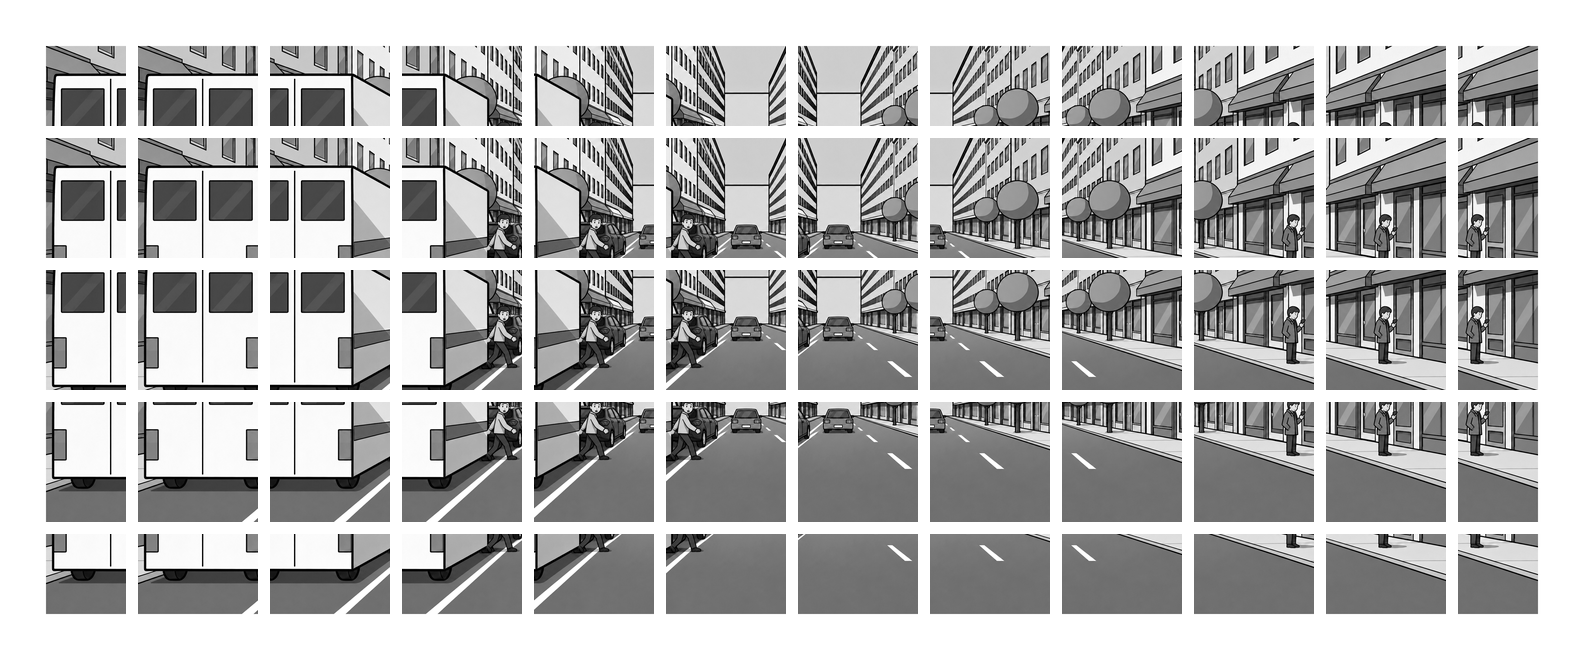
\includegraphics[width=26.4mm]{teaser_assets/patches_dense.png}};
    \foreach \i in {0,...,11} \foreach \j in {0,...,4} \draw[rule, line width=0.25pt] (7.4+\i*\p+0.1, 5.5-\j*\p-0.1) rectangle ++(\q, -\q);
    \foreach \c/\r in \active \draw[actred, line width=0.6pt] (7.4+\c*\p+0.1, 5.5-\r*\p-0.1) rectangle ++(\q, -\q);
    \node[small, anchor=north] at (23.7,-6.0) {receptive fields of \emph{all} positions};
    \node[op] at (35.8,0) {$\otimes$};
    \weights{(38.8,0)}
    \node[op] at (43.0,0) {$=$};
    \node[anchor=north west, inner sep=0] at (44.8,\th/2) {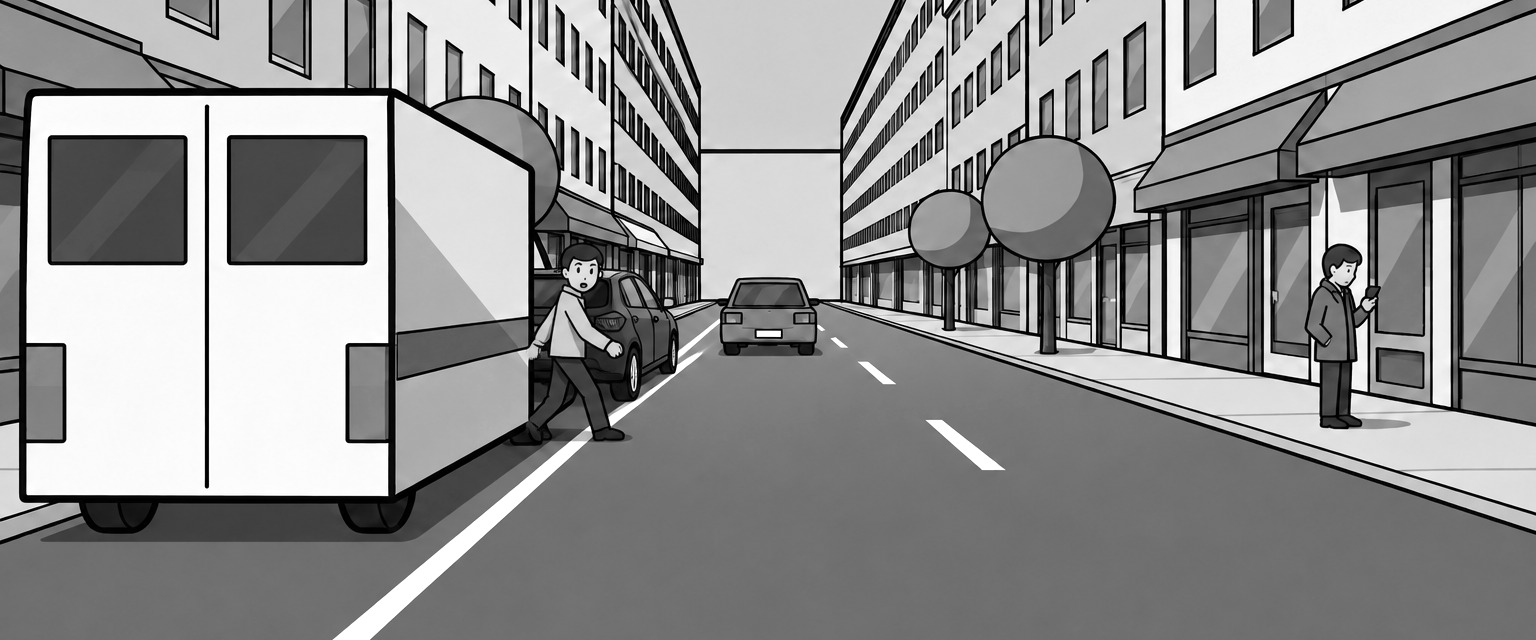
\includegraphics[width=\tw mm]{teaser_assets/scene.jpg}};
    \begin{scope}[shift={(44.8,\th/2)}]
      \draw[detbox] \detbus; \draw[detbox] \detman; \draw[detbox] \detped; \draw[detbox] \detcar;
      \draw[rule, line width=0.4pt] (0,0) rectangle (\tw,-\th);
    \end{scope}
    \node[small, align=center, anchor=north] at (54.3,-4.6) {$\mathbf{y}$: every position\\recomputed};
    \draw[flow] (65.0,0) -- (67.0,0);
    \node[stage] at (71.4,0) {Predict\\\&\\plan};
    \draw[flow] (76.0,0) -- (78.0,0);
    \wheel{(80.4,0)}{baseline}{150/130/2.2, 121/101/2.2, 92/71/0}
    \draw[draw=baseline, line width=0.6pt, dash pattern=on 1.2pt off 0.9pt] (80.4,-2.2) -- (80.4,-36.2);
  \end{scope}
  \draw[baselineframe] (4.6,-48.0) rectangle (65.0,-68.6);
  \node[baselinetag] at (7.4,-48.0) {Baseline: Dense};

  % ---------------- WISEConv ----------------
  \begin{scope}[shift={(0,-78.8)}]
    \fill[smfill, rounded corners=2pt] (6.0,6.6) rectangle (21.6,-12.2);
    \node[smlabel] at (6.0,6.6) {GPU};
    % the active patches sit where their positions lie in the grid (columns 4-6, rows 1-3)
    \node[anchor=north west, inner sep=0] at (7.4,3.3) {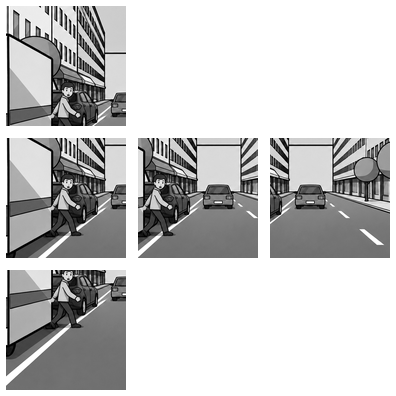
\includegraphics[width=6.6mm]{teaser_assets/patches_ours.png}};
    \foreach \c/\r in \active {
      \draw[rule, line width=0.25pt] (7.4+\c*\p-4*\p+0.1, 3.3-\r*\p+\p-0.1) rectangle ++(\q, -\q);
      \draw[actred, line width=0.6pt] (7.4+\c*\p-4*\p+0.1, 3.3-\r*\p+\p-0.1) rectangle ++(\q, -\q);}
    \node[small, align=center, anchor=north] at (13.8,-4.0) {only \emph{active}\\positions\\(the worklist)};
    \node[op] at (16.0,0) {$\otimes$};
    \weights{(19.0,0)}
    \node[op] at (23.2,0) {$=$};
    \node[anchor=north west, inner sep=0] at (25.0,\th/2) {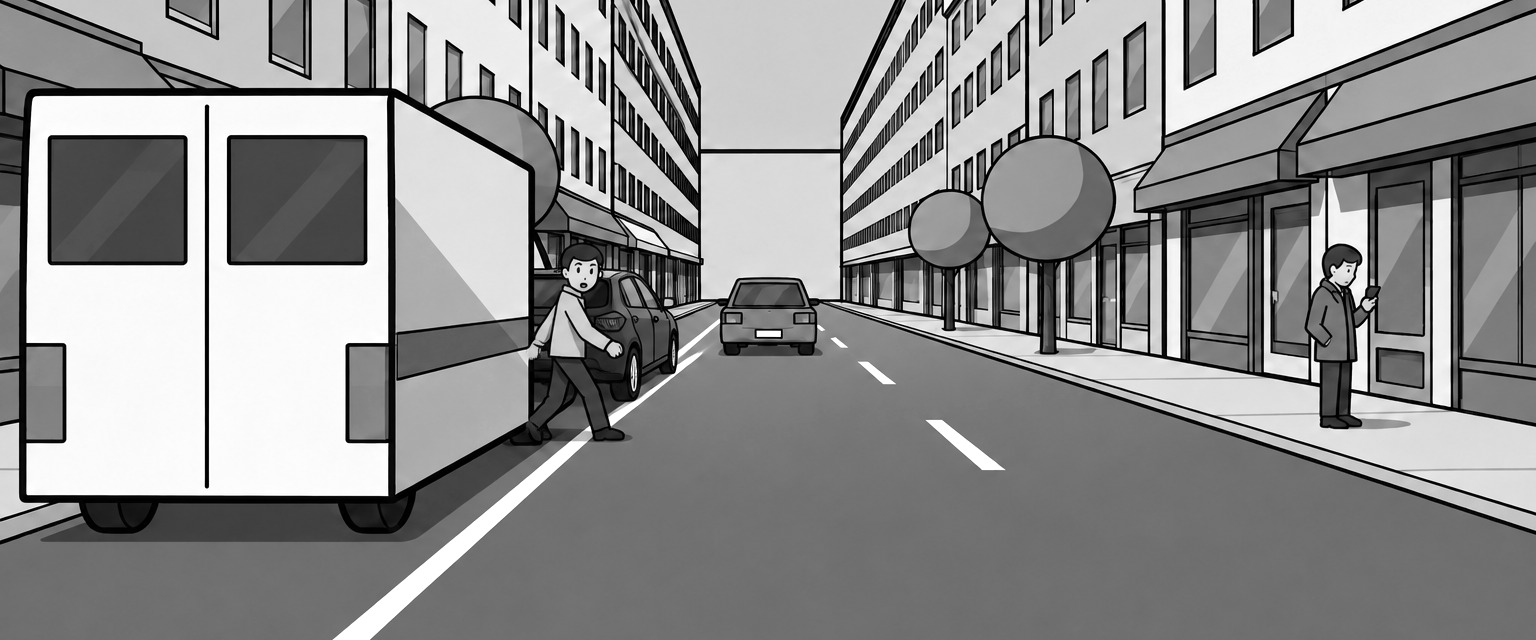
\includegraphics[width=\tw mm]{teaser_assets/scene.jpg}};
    \begin{scope}[shift={(25.0,\th/2)}]
      \path[fill=white, opacity=0.55, even odd rule] (0,0) rectangle (\tw,-\th)
        \foreach \c/\r in \active {(\c*\ts, -\r*\ts) rectangle ++(\ts, -\ts)};
      % outline of the active region only (cells (4,1)-(4,3), (5,2), (6,2))
      \draw[actred, line width=0.6pt] (4*\ts,-1*\ts) -- (5*\ts,-1*\ts) -- (5*\ts,-2*\ts) -- (7*\ts,-2*\ts) -- (7*\ts,-3*\ts)
        -- (5*\ts,-3*\ts) -- (5*\ts,-4*\ts) -- (4*\ts,-4*\ts) -- cycle;
      \draw[reused] \detbus; \draw[reused] \detman; \draw[detbox] \detped; \draw[detbox] \detcar;
      \draw[rule, line width=0.4pt] (0,0) rectangle (\tw,-\th);
    \end{scope}
    \node[small, align=center, anchor=north] at (34.5,-4.6) {$\mathbf{y}$: active recomputed,\\the rest reused};
    \draw[flow] (45.6,0) -- (47.6,0);
    \node[stage] at (52.0,0) {Predict\\\&\\plan};
    \draw[flow] (56.6,0) -- (58.6,0);
    \wheel{(61.0,0)}{wiseconv}{150/71/0}
    \draw[wiseconv, line width=0.6pt, dash pattern=on 1.2pt off 0.9pt] (61.0,-2.2) -- (61.0,-15.4);
  \end{scope}
  \draw[oursframe] (4.6,-71.0) rectangle (45.6,-92.2);
  \node[ourstag] at (7.4,-71.0) {Ours: WISEConv};

  % ---------------- timeline ----------------
  \draw[ink, line width=0.7pt, -{Stealth[length=3pt]}] (4.6,-94.2) -- (\W,-94.2);
  \draw[ink, line width=0.7pt] (4.6,-93.4) -- (4.6,-95.0);
  \node[small, anchor=north west] at (4.0,-94.6) {time};
  \foreach \x/\col/\m in {61.0/ink/-1, 80.4/ink/1} {   % uncolored faces: on time / late
    \begin{scope}[shift={(\x,-97.4)}]
      \draw[\col, line width=0.6pt] (0,0) circle (1.6);
      \fill[\col] (-0.55,0.45) circle (0.22) (0.55,0.45) circle (0.22);
      \draw[\col, line width=0.6pt] (-0.75,{-0.35-0.25*\m}) .. controls (-0.3,{-0.35+0.25*\m}) and (0.3,{-0.35+0.25*\m}) .. (0.75,{-0.35-0.25*\m});
    \end{scope}}
\end{tikzpicture}
\end{document}
